\documentclass{article}
\usepackage[utf8]{inputenc}
\usepackage{microtype}
\usepackage{framed}
\usepackage{todonotes}
\usepackage{wrapfig}
\usepackage{graphicx}
\usepackage{epstopdf}
\usepackage{amssymb,amsmath}
\usepackage{array}
\usepackage{xspace,enumerate}
\usepackage{amsthm}
\usepackage{thmtools}
\usepackage{thm-restate}
\usepackage{verbatim}
\usepackage{mathtools}
\usepackage{sidecap}
\usepackage{svg}
\usepackage{booktabs}
\usepackage{multirow}
\usepackage[font=small,labelfont=bf,skip=1pt]{caption}
\usepackage[ruled, noline, noend, linesnumbered,]{algorithm2e}
%\usepackage{hyperref}
%\usepackage{cleveref}
\usepackage{subcaption}
\usepackage{algpseudocode}
\usepackage[margin=1.65in]{geometry}
\usepackage{pgfplots}
\usepackage{listings}
\usepackage{nicefrac}
\lstset{
  basicstyle=\ttfamily,
 mathescape
}
\usepackage{tikz}
\usetikzlibrary{positioning}
\usetikzlibrary{trees,automata,positioning}
\usetikzlibrary{decorations.pathmorphing}
\usetikzlibrary{decorations.markings}
\usetikzlibrary{decorations.pathmorphing,shapes}
\usetikzlibrary{calc,decorations.pathmorphing,shapes}
\usetikzlibrary{arrows}

\tikzset{
  every node/.style={
    align=center,
    draw=none,
  },
  -latex,
}

\usepackage[colorlinks]{hyperref}
\usepackage[capitalise]{cleveref}

\newcommand{\cS}{\mathcal{S}}
\newcommand{\cG}{\mathcal{G}}
\newcommand{\cF}{\mathcal{F}}
\newcommand{\cX}{\mathcal{X}}
\newcommand{\cP}{\mathcal{P}}
\newcommand{\cM}{\mathcal{M}}
\newcommand{\cI}{\mathcal{I}}
\newcommand{\cL}{\mathcal{L}}
\newcommand{\cO}{\mathcal{O}}
\newcommand{\cT}{\mathcal{T}}
\newcommand{\cC}{\mathcal{C}}
\newcommand{\Tone}{\ensuremath{T_1}}
\newcommand{\Ttwo}{\ensuremath{T_2}}
\newcommand{\Fone}{F_1}
\newcommand{\Ftwo}{F_2}
\newcommand{\ctO}{\tilde{\mathcal{O}}}
\newcommand{\alg}{\textsc{ALG}}
\newcommand{\opt}{\textsc{OPT}}
\newcommand{\nodelabel}{\ell}
\newcommand{\conserved}{\mathsf{conserved}}
\newcommand{\children}{\mathsf{children}}
\newcommand{\head}{\mathsf{head}}
\newcommand{\level}{\mathsf{level}}
\newcommand{\access}{\mathsf{access}}
\newcommand{\mode}{\mathsf{mode}}
\newcommand{\freq}{\mathsf{freq}}
\newcommand{\rep}{\mathsf{rep}}
\newcommand{\dg}{\mathsf{deg}}
\newcommand{\edge}[3]{\ensuremath{#1 | #2 \rightarrow #3}}
\newtheorem{problem2}{Problem}{\bfseries}{\itshape}
\newtheorem{example2}{Example}{\itshape}{\rmfamily}
\newtheorem{example}{Example}
\newtheorem{lemma}{Lemma}
\newtheorem{theorem}{Theorem}
\newtheorem{definition}{Definition}
\newtheorem{fact}[theorem]{Fact}
\newtheorem{observation}[theorem]{Observation}
\SetKwInput{Algorithm}{Algorithm}
\newtheorem{corollary}[theorem]{Corollary}
\newtheorem{conjecture}{Conjecture}
\crefname{hypothesis}{Hypothesis}{Hypotheses}
\newtheorem{problem}{Problem}
\newtheorem{remark}{Remark}

\newcommand{\notaestesa}[2]{%
  \marginpar{\color{red!75!black}\textbf{\texttimes}}%
  {\color{red!75!black}%
    [\,\textbullet\,\textsf{\textbf{#1:}} %
    \textsf{\footnotesize#2}\,\textbullet\,]}%
}
\newcommand{\gdv}[1]{\notaestesa{GDV}{#1:}}
\newcommand{\murray}[1]{\notaestesa{Murray}{#1:}}
\newcommand{\giulia}[1]{\notaestesa{Giulia}{#1:}}

\title{Rearrangement Distances}
\author{giuliabernardini.morg }
\date{November 2020}

\begin{document}

\maketitle

\section{Introduction}\label{sec:trees_motiv}
Phylogenetic trees represent a plausible evolutionary relationship between the most disparate objects: natural languages in linguistics~\cite{gray2009language,walker2012cultural,nakhleh2005comparison}, ancient manuscripts in archaeology~\cite{buneman1971recovery}, genes and species in biology~\cite{huber2006phylogenetic,huson2006application}.
The leaves of such trees are labelled by the entities they represent, while the internal nodes are unlabelled and stand for unknown or extinct items.
A great wealth of methods to infer phylogenies have been developed over the decades~\cite{felsenstein2004inferring,steel2016phylogeny}, together with various techniques to compare the output of different algorithms, e.g., by building a consensus tree that captures the similarity between a set of conflicting trees~\cite{bryant2003classification,jansson2016improved,jansson2016algorithms,DBLP:conf/icalp/GawrychowskiLSW18} or by defining a metric between two trees~\cite{dobson1975comparing,brodal2013efficient,estabrook1985comparison,dudek2019computing,robinson1979comparison,robinson1981comparison}.

Fully-labelled trees, in opposition to classical phylogenies, may model an evolutionary history where the internal nodes, just like the leaves, correspond to extant entities.
An important phenomenon that fits this model well is cancer progressions~\cite{hajirasouliha2014combinatorial,nowell1976clonal}.
With the increasing amount of data and algorithms becoming available for inferring cancer evolution~\cite{malikic2019phiscs,jiao2014inferring,yuan2015bitphylogeny,bonizzoni2018does,bonizzoni2017beyond}, there is a pressing need of methods to provide a meaningful comparison among the trees produced by different approaches.
Besides the well-studied edit distance for fully-labelled trees~\cite{tai1979tree,zhang1989simple,pawlik2015efficient,mcvicar2016sumoted}, a few recent papers proposed ad-hoc metrics for tumor phylogenies~\cite{Karpov2019,govek2018consensus,DiNardo2019,Bioinfo2020}.
Taking inspiration from the existing literature~\cite{dasgupta1997distances, bordewich2005computational, allen2001subtree,steel2016phylogeny} on phylogeny rearrangement, the study of an operational notion of distance for
rearranging a fully-labelled tree is of great interest, and there are still many unexplored questions to be answered.

In this work, we open the investigation of some notions of the
rearrangement distance for two rooted trees which are fully labelled
by the same set of labels.
Building upon the existing
literature~\cite{semple2003phylogenetics,steel2016phylogeny} on
phylogenetic trees rearrangement,  we propose some operations for
rearranging a fully-labelled tree.
The distance between a pair of
trees is then the shortest sequence of these operations that
transforms the first tree into the second tree.
We consider rooted trees on $n$ nodes labelled with distinct labels from $[n]=\{1,2,\ldots,n\}$, and identify nodes with their labels.
The first operation
we introduce is an adaptation of the SPR
operation~\cite{bordewich2005computational} to a fully-labelled tree. We call such an operation \emph{link-and-cut} operation, while the second operation
is a \emph{permutation} of some labels of the tree (notice that such an operation does change the topology of the tree).
When only one kind of operations is allowed, we have the link-and-cut distance and the permutation distance. When both operations are possible, then we have the rearrangement distance.

For computing the permutation distance, in Section~\ref{sec:permutation} we connect the complexity to that of calculating the largest cardinality matching in a sparse bipartite graph. By designing two-way reductions we show that these problems are equivalent, up to polylogarithmic factors.
Due to the recent progress in the area of fine-grained complexity we now know, for many problems that can be solved in polynomial
time, what is essentially the best possible exponent in the running time, conditioned on some plausible but yet unproven
hypothesis~\cite{Williams18}. For max-flow, and more specifically maximum matching, this is not the case yet, although
we do have some understanding of the complexity of the related problem of computing the max-flow between all pairs of
nodes~\cite{AbboudKT20,KrauthgamerT18,AbboudGIKPTUW19}. So, even though our reductions don't tell us what is the best possible
exponent in the running time, they do imply that it is the same as for maximum matching in a sparse bipartite graph.
In particular, by plugging in the asymptotically fastest known algorithm~\cite{liu2020faster}, we obtain an $\ctO(n^{4/3+o(1)})$ time algorithm for computing
the permutation distance between two trees on $n$ nodes. The main technical novelty in our reduction from permutation
distance is that, even though the natural approach would result in multiple instances of weighted maximum bipartite matching,
we manage to keep the graphs unweighted.


In Section~\ref{sec:rearrangement} we show that computing the rearrangement distance between two trees is NP-hard, via a reduction from $3$-dimensional matching~\cite{karp1972reducibility}. In Section~\ref{sec:approxbinary} we consider the special case where one of the two tree is binary and give a simple linear-time $4$-approximation ratio algorithm.
In Section~\ref{sec:approxtree} we design a linear-time constant-factor approximation algorithm that does
not assume that the trees are binary. The algorithm consists of multiple phases, each of them introducing more and
more structure into the currently considered instance, while making sure that we don't pay more than the optimal distance
times some constant. To connect the number of steps used in every phase with the optimal distance, we introduce a new
combinatorial object that can be used to lower bound the latter, inspired by the well-known algorithm
for computing the majority~\cite{Moore91}.
In Section~\ref{sec:fixedpar} we describe a fixed-parameter algorithm for the rearrangement distance.
Finally, in Section~\ref{sec:experiments} we report an experimental analysis that we have run to validate the approximation factor of those algorithms.

\section{Preliminaries}\label{sec:preliminariestree}

Let $[n]=\{1,2,\ldots,n\}$.
Throughout this paper, we consider \emph{fully-labelled}  rooted trees and forests, whose nodes are labelled with distinct labels from $[n]$, and identify nodes with their
labels.
All the problems we consider will have as input two fully-labeled trees or forests such that the set of labels is $[n]$ for both trees (resp. forests), where $n$ is the number of nodes of each input object.
We next introduce the two operations on trees that we will study.


\begin{definition}[link-and-cut operation]
  \label{def:link-and-cut}
Let $u$, $v$, and $w$ be three vertices of a tree $T$,  such that $v$ is a child of $u$ and $w$ is not a descendant of $v$.
Then the link-and-cut operation $v\,|\,u\rightarrow w$ on $T$ consists of a sequence of two operations: first delete from $T$ the edge $(v,u)$, then add the edge $(v,w)$, effectively switching the parent of $v$ from $u$ to $w$.
\end{definition}

%
\begin{definition}[permutation operation]
  \label{def:permutation}
  Let $T$ be a tree and let $\pi:[n]\mapsto [n]$ be a bijective function. 
  The permutation operation defined by $\pi$ consists in applying $\pi$ to $T$, thus changing the label of each node of $T$ labeled by $x$ to $\pi(x)$.
\end{definition}
%

Notice that such a function $\pi$ is a permutation of a subset of $[n]$, where only the labels $x$ such that $\pi(x)\neq x$ are involved in the permutation.
The size $|\pi|$ of a permutation is the number of elements $x$ s.t. $\pi(x)\neq x$.
%Recall that two trees $\Tone$ and $\Ttwo$ are isomorphic if and only if we can reorder the children of every node so as to make the
%trees identical after disregarding the labels.


Given a forest $F$, the parent of $u$ in $F$ is denoted $p_{F}(u)$, and we use the convention
that $p_{F}(u)=\bot$ when $u$ is a root in $F$. Moreover, $F|u$ denotes the subtree of $F$ rooted at $u$,
$\children_{F}(u)$ stands for the set of children of a node $u$ in $F$, and $\level_{F}(u)$ is the level of $u$ in $F$
(the roots have level $0$).
% Two trees $\Tone$ and $\Ttwo$ are \emph{topologically isomorphic}, denoted $\Tone \approx \Ttwo$, if and only if there exists a bijection $\mu$ between their nodes
% such that, for every vertex $v$ of $T_1$, $|\children_{T_1}(v)| = |\children_{T_2}(\mu(v))|$.
Two trees $\Tone$ and $\Ttwo$ are  isomorphic, denoted $\Tone \equiv \Ttwo$, if and only if there exists a bijection $\mu$ between their nodes
such that, for every vertex $u$ of $T_1$,  $\mu(p_{T_{1}}(u))=p_{T_{2}}(\mu(u))$.
Notice that, by this definition, $\mu$ maps the root of $\Tone$ to the root of $\Ttwo$.
% Let $\cI(\Tone,\Ttwo)$ denote the set of all such bijections $\mu$.
% Given two isomorphic trees $\Tone$ and $\Ttwo$, we seek a permutation $\pi$ with the smallest possible size that
% transforms $\Tone$ into $\Ttwo$. This is equivalent to finding $\mu\in\cI(\Tone,\Ttwo)$ that maximises
% the number of conserved nodes $\conserved(\mu)=\{ u :  u = \mu(u) \}$,
% as these two values sum up to $n$.

We now give the  notions of distance between trees
$T_1$ and $T_2$ labelled by $[n]$ that we will study.
Unless otherwise stated, throughout this paper we will assume that the roots of $\Tone$ and $\Ttwo$ have the same label.

\begin{definition}[Distances]
  \label{definition:edge}\label{definition:distances}
Let $T_1$ and $T_2$ be two trees labeled by the set $[n]$.
The \emph{link-and-cut distance} $d_{\ell}(T_1,T_2)$ is the length
of the shortest sequence of link-and-cut operations which transforms
$T_1$ into $T_2$.
\label{definition:rearrangment}
The \emph{rearrangement distance} $d(T_1,T_2)$ is the smallest size of any
sequence of link-and-cut and permutation operations that transforms $T_1$ into $T_2$.
\label{definition:permutation}
If $T_1$ and $T_2$ are isomorphic, then the \emph{permutation distance} $d_{\pi}(T_1, T_2)$ is the size
$|\pi|$ of the smallest permutation $\pi$ that transforms $T_1$ into
$T_2$.
\end{definition}



Clearly, the permutation distance $d_{\pi}(T_1,T_2)$ is defined only
when $T_1$ and $T_2$ are isomorphic, and it is evidently well
posed. The following Lemma ensures that the definition of link-and-cut
distance is well posed too.  
\begin{lemma}
\label{lemma:wellposed}
Given trees $T_1$ and $T_2$ each labelled by $[n]$, there always
exists a sequence of link-and-cut operations that transforms $T_1$
into $T_2$.
\end{lemma}
%
\begin{proof}
For any node $v$, $p_{T_1}(v)=u$, such that $p_{T_2}(v)=w$ and $w$ is
a descendant of $v$ in $T_1$ --- and thus the operation
$\edge{v}{u}{w}$ is not directly applicable --- we prove that there
exists a node $z$ on the path from $v$ to $w$ in $T_1$ (including $w$)
such that $p_{T_2}(z)$ is not a descendant of $v$ in $T_2$ nor a
descendant of $z$ in $T_1$.  This implies that after applying the
valid operation $\edge{z}{p_{T_1}(z)}{p_{T_2}(z)}$, the operation
$\edge{v}{u}{w}$ becomes valid too.  There is always such a node $z$
because, should it not exist, $w$ would be a descendant of $v$ also in
$T_2$, giving rise to the cycle $(w \rightarrow v \rightarrow \cdots
\rightarrow w)$ and thus contradicting the fact that $T_2$ is a tree.
\end{proof}

Since these operations are invertible,
all the above distance measures are symmetric. Moreover, they satisfy by
definition the triangle inequality.
% : consider, e.g., the rearrangement
% distance. Given $T_1$, $T_2$ and $T_3$ labelled by the same set of
% labels, let $\cS_{12}$ be a sequence that transforms $T_1$ into $T_2$
% such that $|\cS_{12}|=d(T_1,T_2)$, $\cS_{23}$ a sequence that
% transforms $T_2$ into $T_3$ with $|\cS_{23}|=d(T_2,T_3)$, $\cS_{13}$ a
% sequence that transforms $T_1$ into $T_3$ and $|\cS_{13}|=d(T_1,T_3)$.
% It is evident that the concatenation $\cS_{12} \cS_{13}$ of $\cS_{12}$
% and $\cS_{23}$ is a sequence that transforms $T_1$ into $T_3$, and by
% Definition~\ref{definition:rearrangment} its size is larger or equal to
% $d(T_1,T_3)$: thus $d(T_1,T_2) + d(T_2,T_3) \ge |\cS_{12} \cS_{23}|\ge
% d(T_1,T_3)$.  A similar argument shows that the triangular inequality
% also holds for the link-and-cut distance and the permutation distance.

%We next define two structures that capture two fundamental characteristics of the trees to compare.

% \begin{definition}[active set]
%   \label{definition:active}
%   Given trees $T_1$ and $T_2$, we call
%   \emph{active} the subset $\cX \subseteq [n]$ of labels which have
%   different parents in $T_1$ and $T_2$, i.e., $v \in \cX$ iff
%   $p_{T_1}(v) \ne p_{T_2}(v)$.
% \end{definition}
In Section~\ref{sec:approxtree}, for ease of presentation, in addition to the link-and-cut operation we will also work with the cut operation, defined as follows:
\begin{definition}
[cut operation] Let $u,v$ be two nodes such that $v$ is a child of $u$. The cut operation
$(v\dagger u)$ removes the edge $(v,u)$, effectively making $v$ a root and $u$ a leaf.
\end{definition}
The size of a sequence of cut and permutation operations is defined similarly as for a sequence
of link-and-cut and permutation operations.
Since a permutation operation is essentially just renaming the nodes, we can assume
that all permutation operations precede all link-and-cut (or cut) operations, or vice versa.
Furthermore, consecutive permutation operations that are not pairwise disjoint can be replaced by a single permutation operation
without increasing the total size.

This leads to the notion of rearrangement distance between two forests $\Fone$ and $\Ftwo$.
We write $\Fone\sim \Ftwo$ to denote that, for every $u\in [n]$, at least one of the following three conditions holds:
(i) $p_{\Fone}(u) = p_{\Ftwo}(u)$,
(ii) $p_{\Fone}(u)=\bot$, or
(iii) $p_{\Ftwo}(u)=\bot$.
The rearrangement distance $\tilde{d}(\Fone,\Ftwo)$ is the
smallest size of any sequence of cut and permutation operations that transforms $\Fone$ into $\Fone'$ such that $\Fone' \sim \Ftwo$.
This is the same as the smallest size of any sequence of cut and permutation operations
that transforms $\Ftwo$ into $\Ftwo'$ such that $\Fone \sim \Ftwo'$, as both sizes are equal
to the minimum over all permutations $\pi$ that fix the original root of the following expression
\[ |\{ u : \pi(u) \neq u\}| + |\{ u : p_{\Fone}(u) \neq p_{\Ftwo}(\pi(u))~\land~p_{\Fone}(u)\neq \bot~\land~p_{\Ftwo}(\pi(u))\neq \bot \}| . \]
Consequently, $\tilde{d}$ defines a metric.
%The original notion of rearrangement distance $d$ between two trees is similarly defined as the smallest size of any sequence of link-and-cut and permutation operations that transforms $\Tone$ into $\Ttwo$, under the additional assumption that the roots of
%$\Tone$ and $\Ttwo$ are identical (so $d(\Tone,\Ttwo)$ is well-defined) and cannot participate in any
%permutation operation.
In Section~\ref{sec:approxtree} we connect $d(\Tone,\Ttwo)$ and $\tilde{d}(\Tone,\Ttwo)$, and then work with the latter.

A matching in a bipartite graph is a subset of edges with no two edges meeting at the same vertex. A maximum matching
in an unweighted bipartite graph is a matching of maximum cardinality, whereas a maximum weight matching in a weighted
bipartite graph is a matching in which the sum of weights is maximised.
Given an unweighted bipartite graph with $m$ edges, the well-known algorithm by Hopcroft and Karp~\cite{HopcroftK73} finds
a maximum matching in $\cO(m^{1.5})$ time. This has been recently improved by Liu and Sidford to $\tilde\cO(m^{4/3+o(1)})~$\cite{liu2020faster}.

A \emph{heavy path decomposition} of a tree $T$ is obtained by selecting, for every non-leaf node $u\in T$, its \emph{heavy child} $v$ such
that $T|v$ is the largest: there will be some subtlety in how to resolve a tie in this definition that will be explained in detail later.
This procedure decomposes the nodes of $T$ into node-disjoint paths called \emph{heavy paths}.
Each heavy path $p$ starts at some node, called its \emph{head}, and ends at a leaf: $\head_{T}(u)$ denotes the head of the heavy path containing a node $u$ in $T$. An important property of such a decomposition is
that the number of distinct heavy paths above any leaf (that is, intersecting the path from a leaf to the root) is only logarithmic
in the size of $T$~\cite{DBLP:journals/jcss/SleatorT83}.

\section{Link-and-cut Distance}
\label{sec:link-and-cut}

In this section we present a simple linear-time algorithm to compute the link-and-cut distance between two trees.  
\begin{comment}
The main technical device is called \emph{family partition}.\giulia{We do not really need to define the family partition in this section, I think. }

Given two trees $T_1$ and $T_2$, we can associate with $v$ the pair
$(p_{T_1}(v),p_{T_2}(v))$ of the parents of $v$ in the two trees.
Given a pair of (not necessarily distinct) nodes $u$ and $w$, we
define $\cP_{(u,w)}$ as the set $\{v ~:~ p_{T_1}(v) = u, ~ p_{T_2}(v)
= w\}$.\giulia{Does it make sense to define it for $u=w$, when in $\mathcal{P}$ we only consider the sets with $u\neq w$? Also,  $\mathcal{P}$ was a partition of the active set, but now it does not partition anything. We should at least change the name}  Since each vertex different from the root has exactly one
parent in each tree, each vertex $v\in [n]$ belongs to exactly one set $\cP_{(u,w)}$.
This fact leads to the following definition, which is illustrated in
Example~\ref{ex:partition}.

\begin{definition}[family partition]
  \label{definition:partition}
  Let trees $T_1$ and $T_2$ each be labelled by $[n]$: for each vertex
  $v \in [n]$ we denote the set $\cP_{(u,w)} = \{v ~:~ p_{T_1}(v) = u,
  ~ p_{T_2}(v) = w\}$.  Then $\cP$, called \emph{family partition}, is the collection of the nonempty sets $\cP_{(u,w)}$, $u,w \in V$ such that $u\neq w$.
\end{definition}

\begin{example}
  \label{ex:partition}
  Consider $T_1$ and $T_2$ of Figure~\ref{fig:dist}.
  The family partition is composed of the
  following sets: $\cP_{(2,3)}=\{4,5,6\}$, $\cP_{(3,2)}=\{10\}$.
\end{example}
\end{comment}
\begin{figure}[t]
    \centering
   \includegraphics[width=0.95\linewidth]{Fig/rearrangement.pdf}
    \caption[Example of rearrangement distance between two trees]{Trees $\Tone$ and $\Ttwo$ labelled by $[10]$. The link-and-cut distance $d_\ell(\Tone,\Ttwo)$ is 4, given, for example, by the sequence $\edge{4}{2}{3}$, $\edge{5}{2}{3}$, $\edge{6}{2}{3}$, $\edge{10}{3}{2}$. The rearrangement distance is 3, given, for example, by the sequence $(2~3),\edge{7}{3}{2}$.}
    \label{fig:dist}
  \end{figure}


%
%
%The following Lemma explicits the relevance of the notion of family partition.

\begin{lemma}
\label{lemma:algorithm-link-and-cut}
Given two trees $T_1$ and $T_2$ each labelled by $[n]$, let $X$ be the set of nodes $v$ such that $p_{T_1}(v) \neq p_{T_2}(v)$. 
Then $d_\ell(T_1, T_2)= |X|$ and a sequence of $|X|$ link-and-cut operations that transforms $T_1$ into $T_2$ can be computed in linear time.
%there is a linear-time algorithm that computes the shortest sequence of link-and-cut operations that transforms $T_1$ into $T_2$, and such a sequence consists of $|X|$ operations.
\end{lemma}
%
\begin{proof}
 % In this proof we will exploit the fact that no two nodes of a tree share the same label by using a label to denote a node --- we will make the tree explicit when necessary.\giulia{I removed this because in the preliminaries we already say that we identify the nodes with their labels.}

  Let $v$ be a node in $X$. %, that is $v$ belongs to a set $\cP_{(a,b)}$ with $a\neq b$.
  Notice that each node in $X$ must be moved with at least a link-and-cut operation, hence $d_\ell(T_1, T_2)\ge |X|$. In the following we will describe how to obtain a sequence of exactly $|X|$ operation transforming $T_1$ into $T_2$.

  Let $v$ be a node of $X$ such that no proper descendant of $v$ in $T_1$ belongs to $X$ --- if no such node $v$ exists, then $T_1$ and $T_2$ are isomorphic. \giulia{I do not understand the previous claim. How can such $v$ not exist? Only if $X$ is empty, but then the two trees are equal.}
  Without loss of generality, let $p_{T_1}(v)=u$ and $p_{T_2}(v)=w$.

  We claim that $w$ is never a descendant of $v$ in $T_1$, and we can therefore apply the $\edge{v}{u}{w}$ operation --- hence removing $v$ from $X$ --- and recurse on the resulting tree.
  In fact, assume for a contradiction that $w$ is a descendant of $v$ in $T_1$, and let $<v, x_1, \ldots, x_{q-1}, x_q = w>$ be the path of $T_1$ from $v$ to $w$. Since no proper descendant of $v$ in $T_1$ belongs to $X$, $p_{T_1}(x_i)=p_{T_2}(x_i)$ for each $i\le q$, that is $<v, x_1, \ldots, x_{q-1}, x_q = w>$ is also a path of $T_2$, implying that $v$ is an ancestor of $w$ in $T_2$ as well. 
  This contradicts the fact that $p_{T_2}(v)=w$, therefore $w$ is not a descendant of $v$ in $T_1$ and the link-and-cut operation $\edge{v}{u}{w}$ is valid.  

  The time complexity is a consequence of the fact that a visit of the two trees $T_1$ and $T_2$ suffices to determine $p_{T_1}(x)$ and $p_{T_2}(x)$ for all $x\in[n]$ and the order in which the operations can be applied.
  \end{proof}

  
% Note that the family partition encodes the elements of any shortest
% sequence of link-and-cut operations for transforming $T_1$ into $T_2$:
% $v \in \cP_{(u,w)}$ corresponds to operation $\edge{v}{u}{w}$. It is
% easy to see, from the proof of Lemma~\ref{lemma:wellposed}, that a
% shortest sequence of valid link-and-cut operations can be obtained from
% $\cP$ by ordering the set of operations it encodes with respect to a
% \emph{depth-first traversal} (DFT) of $T_1$:
% $\edge{u}{p_{T_1}(u)}{p_{T_2}(u)}$ precedes
% $\edge{v}{p_{T_1}(v)}{p_{T_2}(v)}$ if $u$ precedes $v$ in a DFT of
% $T_1$. Hence the link-and-cut distance $d_{\ell}(T_1,T_2)$
% is equal to number of nodes that are in some set of the family partition  $\cP$.

\section{Permutation Distance}
\label{sec:permutation}
Our aim is to find an isomorphic map $\mu\in\cI(\Tone,\Ttwo)$ that maximises $\conserved(\mu)$, that is
$\gamma(\Tone,\Ttwo)=\max \{ \conserved(\mu) : \mu \in \cI(\Tone,\Ttwo)\}$. To make the notation less
cluttered, we define $\gamma(x,y)=\gamma(\Tone|x,\Ttwo|y)$.
Let us start by describing a simple polynomial time algorithm which illustrates the basic idea behind the procedure.
We will then show how to improve it to obtain a faster algorithm that uses unweighted bipartite maximum matching.
Finally, we will show a reduction from bipartite maximum matching to computing
the permutation distance, establishing that these two problems are in fact equivalent, up to polylogarithmic factors.

\subsection{Polynomial Time Algorithm }\label{subsec:n2}

The first step of our solution is to run the folklore linear-time algorithm of Aho et al.~\cite{Aho} for determining if two rooted trees are isomorphic.
Recall that this algorithm assigns a number from $\{1,2,\ldots,2n\}$ to every node of $\Tone$ and $\Ttwo$ so that the subtrees
rooted at two nodes are isomorphic if and only if their numbers are equal.
The high-level idea is then to consider a weighted bipartite graph
$G(u,v)$ for each $u,v\in [n]$ such that $\level_{\Tone}(u)=\level_{\Ttwo}(v)$ and $\Tone|u \equiv \Ttwo|v$.
The vertices of $G(u,v)$ are $\children_{\Tone}(u)$ and $\children_{\Ttwo}(v)$, and there is
an edge of weight $\gamma(u',v')$ between $u' \in \children_{\Tone}(u)$ and $v' \in \children_{\Ttwo}(v)$ if and only if
$\Tone|u' \equiv \Ttwo|v'$ and $\gamma(u',v')>0$.
We call such graphs the \emph{distance graphs} for $\Tone$ and $\Ttwo$ and denote them collectively by $\cG(\Tone,\Ttwo)$. See Figure~\ref{fig:graphs}
 for an example.

The weights $\gamma(u,v)$ are computed as follows, with $\cM(G(u,v))$ denoting the weight of
a (not necessarily perfect) maximum weight matching in $G(u,v)$, and $\Gamma:[n]\times[n]\rightarrow\{0,1\}$ being a function such that $\Gamma(u,v)=1$ if $u=v$ and $\Gamma(u,v)=0$ otherwise.
\begin{equation}
\label{eq:recursion}
  \gamma(u,v) = \left\{
    \begin{array}{ll}
      \cM(G(u,v))+ \Gamma(u,v) & \textrm{ if } T_1|u \equiv T_2|v,\\
      0 & \textrm{ otherwise.}\\
    \end{array}
  \right.
\end{equation}
Note that the overall number of edges created in all graphs is $\cO(n^2)$. Indeed, for each $u\in [n]$
such that $\level_{\Tone}(u)=\level_{\Ttwo}(u)$ and $\Tone|u \equiv \Ttwo|u$,
and for each pair of ancestors $z$ of $u$ in $\Tone$ and $w$ of $u$ in $\Ttwo$ such that $\level_{\Tone}(z)=\level_{\Ttwo}(w)$ and
$\Tone|z \equiv \Ttwo|w$, we possibly add an edge $(z,w)$ to the graph $G(p_{\Tone}(z),p_{\Ttwo}(w))$.
Since there are up to $n$
pairs of ancestors on the same level for each label, and the labels are $n$, there are $\cO(n^2)$ edges overall.

We then start from the deepest level in both trees, and we move up level by level
towards the roots in both trees simultaneously. For each level $k$, we consider all pairs of isomorphic subtrees rooted at level $k$,
build the corresponding distance graphs, and use Equation (\ref{eq:recursion}) to weigh the edges. After having reached the roots, we
return the value of $\gamma(\Tone,\Ttwo)$. The correctness of the algorithm is given by the following lemmas, the first one stating that the permutation distance is equal to the minimum number of labels that are not conserved by any isomorphic mapping.

\begin{lemma}\label{lem:gamma}
For any two isomorphic trees $\Tone$, $\Ttwo$, each labelled by $[n]$, it holds that $d_{\pi}(\Tone,\Ttwo)=n-\gamma(\Tone,\Ttwo)$.
\end{lemma}
\begin{proof}
  Consider an isomorphic mapping $\mu$ from $T_1$ to $T_2$ that has the
  minimum number of mismatched labels $\Delta(\mu) = n-\gamma(\Tone,\Ttwo)$ and consider the set of labels of the vertices involved in the
  set of mismatching vertices given by
  $\mu$.

  Clearly, such labels are in a permutation $\pi$ which rearranges the
  labels of tree $T_1$ to obtain $T_2$, while, by construction of $\mu$,
  all the other labels will not be perturbed by $\pi$.  Then we need
  to show that such a permutation rearranges the minimum number of
  distinct labels, that is, its size $|\pi| = d_{\pi}(T_1, T_2)$ is
  the permutation distance.  Indeed, assume to the contrary that the
  permutation distance $d_{\pi}(T_1,T_2) < |\pi|$.  This implies the
  existence of a permutation $\pi'$ that rearranges fewer labels than
  $\pi$, i.e., $|\pi'| < |\pi|$.  Then we show that there exists an
  isomorphic mapping $\mu'$ that has mismatch number less than the one
  of $\mu$, contradicting the initial assumption.

  Indeed, consider the permutation $\pi'$ and define the mapping $\mu'$
  from $T_1$ to $T_2$ such that $\mu'(u) = v$ whenever $\pi'(v) = u$ The
  mapping $\mu'$ is an isomorphism by the construction of $\pi'$, since
  $\mu'(\pi'(u)) = u$ for all nodes $u$ of $\Tone$, and with the application
  of $\pi'$, the two trees are congruent, hence congruency of the
  labels implies isomorphism of the two trees.  This concludes the
  proof that $\mu'$ is an isomorphism thus leading to a contradiction.
\end{proof}

\begin{lemma}
Recursion~\ref{eq:recursion} is correct.
\end{lemma}
\begin{proof}
 It is essentially a proof by induction. Recall that $\gamma(u,v)$ is the maximum number of labels conserved by any isomorphism between $\Tone|u$ and $\Ttwo|v$. If both $u$ and $v$ are
leaves, then $T_1|u \equiv T_2|v$ is trivially true and
$\gamma(u,v) = \Gamma(u,v)$.  When $T_1|u \equiv T_2|v$ does not hold,
then the permutation distance (thus $n-\gamma(u,v)$, by Lemma~\ref{lem:gamma}) is undefined.

Otherwise, if $u$ and $v$ are internal vertices, and
$T_1|u \equiv T_2|v$, then let $\mu$ be a bijective mapping from the
nodes of $T_1|u$ to the nodes of $T_2|v$ maximizing $\conserved(\mu)$.
By the definition of $\gamma$ and the construction of $\mu$, $\gamma(u,v)=\sum_{z\in\children(u)}\gamma(z,\mu(z)) + \Gamma(u,v)$.
By the inductive hypothesis, all values $\gamma(z,\mu(z))$ are correctly computed; since $\mu$ is the bijective mapping maximizing the conserved labels, no other mapping $\mu'$
can achieve a larger value of $\sum_{z\in\children(u)}\gamma(z,\mu(z))$, and so $\mu(z)$ is determined by a maximum weight matching on $G(u,v)$.
\end{proof}

The running time is polynomial if we plug in any polynomial-time maximum weight matching algorithm.

In the next subsection we show how to obtain a better running time by constructing a different version of distance graphs, so that the total weight of their edges will be subquadratic,
and replacing maximum weight matching with maximum matching.

\subsection{Reduction to Bipartite Maximum Matching}
\label{sub:reduction}
We start by finding a heavy path decomposition of $\Tone$ and $\Ttwo$, with some extra care in resolving a tie if there are multiple children with subtrees of the same size, as follows.
Recall that we already know which subtrees of $\Tone$ and $\Ttwo$ are isomorphic, as the algorithm of~\cite{Aho} assigns the same number from $\{1,2,\ldots,2n\}$ to nodes of $\Tone$ and $\Ttwo$ with isomorphic subtrees.
For every $u,v\in [n]$ such that $\Tone|u \equiv \Ttwo|v$, we would like the heavy child $u'$ of $u$ in $\Tone$
and $v'$ of $v$ in $\Ttwo$ to be such that $\Tone|u' \equiv \Ttwo|v'$.
This can be implemented in linear time: it suffices to group the
nodes with isomorphic subtrees together, and then make the choice just once for every such group.

Consider a graph $G(u,v)$ for some $u,v\in [n]$: the edge corresponding to the heavy child $u'$ of $u$ in $\Tone$
and the heavy child $v'$ of $v$ in $\Ttwo$ is called \emph{special} (note that this edge might not exist).
The key observation is that the properties of heavy path decomposition
allow us to bound the total weight of non-special edges by $\cO(n\log n)$.

\begin{figure}[t]
    \centering
   \includegraphics[width=0.9\linewidth]{Fig/Tone_Ttwo.pdf}
    \caption[Example of heavy path decomposition]{$\Tone$ and $\Ttwo$ with a possible heavy path decomposition.}
    \label{fig:paths}
\end{figure}

\begin{figure}
\centering
    \begin{subfigure}[height=2.5cm]{0.38\textwidth}
        \includegraphics[width=\linewidth]{Fig/graphs.pdf}
    \end{subfigure}
    ~~~~~~
    \begin{subfigure}[height=2.5cm]{0.13\textwidth}
        \includegraphics[width=\linewidth]{Fig/G1aa.pdf}
    \end{subfigure}
     ~~~~~~
    \begin{subfigure}[height=2.5cm]{0.13\textwidth}
        \includegraphics[width=\linewidth]{Fig/G2aa.pdf}
    \end{subfigure}

    \caption[Graphs of type 1 and type 3]{$G(a,a)$ (type 1), $G'(a,a)$, $G''(a,a)$ and $G(b,c)$ (type3) for the trees of Figure~\ref{fig:paths}. The special edge in each graph is dashed.}
    \label{fig:graphs}
\end{figure}

\begin{lemma}
\label{lem:nonspecial}
The total weight of all non-special edges in $\cG(\Tone,\Ttwo)$ is $\cO(n\log n)$.
\end{lemma}

\begin{proof}
Consider any $u\in [n]$ such that $\level_{\Tone}(u)=\level_{\Ttwo}(u)$ and $\Tone|u \equiv \Ttwo|u$.
For each pair of ancestors $z$ of $u$ in $\Tone$ and $w$ of $u$ in $\Ttwo$ such that $\level_{\Tone}(z)=\level_{\Ttwo}(w)$,
$\Tone|z \equiv \Ttwo|w$ and either $\head_{\Tone}(z)=z$ or $\head_{\Ttwo}(w)=w$, $u$ will contribute 1 to the weight of an edge $(z,w)$ in $G(p_{\Tone}(z),p_{\Ttwo}(w))$.
Because there are at most $\log n$ heavy paths above
any node of $\Tone$ or $\Ttwo$, each label $u\in [n]$ contributes 1 to the weight of at most $2\log n$ non-special edges, making their total weight $\cO(n\log n)$ overall.
\end{proof}

Recall that $\Gamma:[n]\times[n]\rightarrow\{0,1\}$ is a function such that $\Gamma(u,v)=1$ if $u=v$ and $\Gamma(u,v)=0$ otherwise. We divide the graphs in $\cG(\Tone,\Ttwo)$ into three types (see Figure~\ref{fig:graphs}, left, for an example):
\begin{description}
\item[Type 1: ] graphs $G(u,v)$ with at least one non-special edge.
\item[Type 2: ] graphs $G(u,v)$ with no non-special edges, and $\Gamma(u,v)=1$.
\item[Type 3: ] graphs $G(u,v)$ with no non-special edges, and $\Gamma(u,v)=0$.
\end{description}

We will construct only the graphs of type 1 and 2, and extract from them the information that the graphs of type 3 would have captured.
In what follows we show  how to construct the graphs of type 1 and 2 in $\cO(n\log^{2} n)$ time.

\paragraph{Constructing the graphs of type 1 and 2.}\label{subsub:constructing}
The first step is to find all pairs of nodes that correspond to graphs of type 1 or 2, and store them
in a dictionary $D$ implemented as a balanced search tree with $\cO(\log n)$ access time.
The second step is to find the non-special edges of these graphs, and store them in a separate dictionary, also implemented as a balanced search tree with $\cO(\log n)$ access time.
Note that the weights will be found at a later stage of the algorithm.
We assume that both trees have been already decomposed into heavy paths, and we already know which subtrees are isomorphic.
This can be preprocessed in $\cO(n)$ time.

\begin{lemma}
All graphs of type 1 and 2 can be identified in $\cO(n\log^2 n)$ time.
\end{lemma}

\begin{proof}
We consider every $u\in [n]$ such that $\level_{\Tone}(u)=\level_{\Ttwo}(u)$
and $\Tone | u \equiv \Ttwo | u$ in two passes. In the first pass,
we need to iterate over every ancestor $z$ of $u$ in $\Tone$
and $w$ of $u$ in $\Ttwo$ such that $\level_{\Tone}(z)=\level_{\Ttwo}(w)$, $T_{1}|z \equiv T_{2}|w$ and either $\head_{\Tone}(z)=z$ or $\head_{\Ttwo}(w)=w$,
and if additionally $T_{1}|p_{T_{1}}(z) \equiv T_{2}|p_{T_{2}}(w)$ then designate $G(p_{T_{1}}(z),p_{T_{2}}(w))$ to be a graph of type 1 and insert it into $D$.
As a non-special edge $(z,w)$ of a graph $G(p_{T_{1}}(z),p_{T_{2}}(w))$ is such that either $z$ or $w$ are not on the same heavy path as their parents, this correctly determines all graphs of type 1.

To efficiently iterate over all such $z$ and $w$ given $u$,
we assume that the nodes of every heavy path of a tree $T$ are stored in an array, so that, given any node $u\in T$, we are able to access the node that belongs to the same heavy path as $u$ and whose level is $\ell$ in constant time, if it exists.
We denote such operation $\access_{T}(u,\ell)$.
Given two nodes $u\in\Tone$ and $v\in\Ttwo$ on the same level, the procedure above shows how to iterate over every ancestor $z$ of $u$ and $w$ of $v$ such that $\level_{\Tone}(z)=\level_{\Ttwo}(w)$ and either $\head_{\Tone}(z)=z$ or $\head_{\Ttwo}(w)=w$, in $\cO(\log n)$ time,
implying that all graphs of type 1 can be identified in $\cO(n\log^{2}n)$ time.
{
\setlength{\interspacetitleruled}{0pt}%
\setlength{\algotitleheightrule}{0pt}%
\begin{algorithm}[tb]
\While{$u \neq \bot$ {\bf and} $v\neq \bot$}{
  \uIf{$ \level_{T_{1}}(\head_{T_{1}}(u)) < \level_{T_{2}}(\head_{T_{2}}(v)) $}{
    output $\access_{T_{1}}(u,\level_{T_{2}}(\head_{T_{2}}(v)))$ and $\head_{T_{2}}(v)$\;
    $v \gets p_{T_{2}}(\head_{T_{2}}(v))$\;
  }\eIf{$ \level_{T_{1}}(\head_{T_{1}}(u)) > \level_{T_{2}}(\head_{T_{2}}(v)) $}{
    output $\head_{T_{1}}(u)$ and $\access_{T_{2}}(v,\level_{T_{1}}(\head_{T_{1}}(u)))$\;
    $u \gets p_{T_{1}}(\head_{T_{1}}(u))$\;
  }{
    output $\head_{T_{1}}(u)$ and $\head_{T_{2}}(v)$\;
    $u \gets p_{T_{1}}(\head_{T_{1}}(u))$\;
    $v \gets p_{T_{2}}(\head_{T_{2}}(v))$\;
  }
}
\end{algorithm}
}

In the second pass,
for each $u\in [n]$ such that $\level_{\Tone}(u)=\level_{\Ttwo}(u)$
and $\Tone | u \equiv \Ttwo | u$, we designate $G(u,u)$ to be a graph of type 2, unless it has been already designated to be a graph of type 1.
\end{proof}

\begin{lemma}
All graphs of type 1 and 2 can be populated with their edges in $\cO(n\log^2 n)$ time.
\end{lemma}

\begin{proof}
For each such graph $G(u,v)$ such that none of $u,v$
is a leaf, let $u'$ be the unique heavy child of $u$, and $v'$ be the unique heavy child of $v$. We add the special
edge $(u',v')$ to $G(u,v)$. To find the non-special edges, we again consider every $u\in [n]$ such that
$\level_{\Tone}(u)=\level_{\Ttwo}(u)$ and $\Tone|u \equiv \Ttwo|u$: we iterate over the ancestors $z$ of $u$ in $\Tone$
and $w$ of $u$ in $\Ttwo$ such that $\level_{\Tone}(z)=\level_{\Ttwo}(w)$, $T_{1}|z \equiv T_{2}|w$ and either $\head_{\Tone}(z)=z$ or $\head_{\Ttwo}(w)=w$, and if additionally $T_{1}|p_{\Tone}(z) \equiv T_{2}|p_{\Ttwo}(w)$ then add a non-special edge
$(z,w)$ to $G(p_{\Tone}(z),p_{\Ttwo}(w))$ .
This takes $\cO(n\log^{2}n)$ time overall.
\end{proof}

\paragraph{Processing the graphs of type 1 and 2.}\label{subsub:processing}
Having constructed the graphs of type 1 and 2 in $\cO(n\log^{2}n)$ time, we process them level by level.
Consider $G(u,v)$: for each of its edges $(u',v')$ corresponding to $u'\in\children_{T_{1}}(u)$
and $v'\in\children_{T_{2}}(v)$, we need to extract its weight $\gamma(u',v')$. If $G(u',v')$ is of type 1 or 2,
the graph
can be extracted from the dictionary in $\cO(\log n)$ time. Otherwise,
$G(u',v')$ is of type 3 and we need to make up for not having processed such graphs.

To this aim, we associate a sorted list of levels with each pair of heavy paths of $\Tone$ and $\Ttwo$.
The lists are stored in a dictionary indexed by the heads of the heavy paths.
For every $u,v\in[n]$ such that $G(u,v)$ is of type 1 or 2, we append
the levels of $u$ and $v$ to the lists associated with the respective heavy paths.
The lists can be constructed in $\cO(n\log^{2}n)$ time by processing the graphs level by level, and allow us to efficiently use the following lemma.

\begin{lemma}
\label{lem:type3}
Consider $u,v\in [n]$ such that $\level_{\Tone}(u)=\level_{\Ttwo}(v)$ and $\Tone|u\equiv \Ttwo|v$,
but $G(u,v)$ is of type 3. Either both $u$ and $v$ are leaves and $\gamma(u,v)=0$,
or the heavy child of $u$ is $u'$, the heavy child of $v$ is $v'$, and $\gamma(u,v)=\gamma(u',v')$.
\end{lemma}

\begin{proof}
First observe that $u\neq v$, as otherwise $G(u,v)$ would be of type 2.
Becase $\Tone|u\equiv \Ttwo|v$, either both $u$ and $v$ are leaves or none of them is a leaf.
In the former case, $G(u,v)$ is empty and $\gamma(u,v)=0$.
By how we resolve ties in the heavy path decomposition, in the latter case we have $\Tone|u' \equiv \Ttwo|v'$,
where $u'$ is the heavy child of $u$ and $v'$ is the heavy child of $v$.
$G(u,v)$ consists of the unique special edge corresponding to the heavy child $u'$ of $u$
and $v'$ of $v$, so $\cM(G(u,v))$ is equal to the
cost of the special edge, and by Equation~\ref{eq:recursion} we obtain that $\gamma(u,v)=\gamma(u',v')$.
\end{proof}

Given $u,v\in [n]$ such that $\level_{\Tone}(u)=\level_{\Ttwo}(v)=\ell$ and $\Tone|u\equiv \Ttwo|v$,
we extract $\gamma(u,v)$ by accessing the sorted list associated with the heavy paths of $u$ and $v$: we binary search for the smallest level $\ell'\geq \ell$ such that the heavy paths of $u$ and $v$ respectively contain a node
$u'$ and $v'$, both on level $\ell'$, with $G(u',v')$ of type
1 or 2. Then Lemma~\ref{lem:type3}, together with the fact that in our heavy path decomposition the subtrees rooted at
the heavy children of two nodes with isomorphic subtrees are also isomorphic, implies that
$\gamma(u,v)=\gamma(u',v')$.

It remains to describe how to compute $\cM(G(u,v))$ for every graph $G(u,v)$ of type 1 and 2. We could
have used any maximum weight matching algorithm, but this would result in a higher running time.
Our goal is to plug in a maximum unweighted matching algorithm. This seems problematic as $G(u,v)$ is a weighted
bipartite graph, but we will show that maximum weight matching can be reduced to multiple instances
of maximum matching. However, bounding the overall running time will require bounding the total weight
of all edges belonging to graphs of type 1 and 2. By Lemma~\ref{lem:nonspecial} we already know that the total
weight of all non-special edges is $\cO(n\log n)$, but such bound doesn't hold for the special edges.
Therefore, we proceed as follows. Let $u'$ be the heavy child of $u$ and $v'$ be the heavy child of $v$.
We construct $G'(u,v)$ by removing the special edge from $G(u,v)$.
We also construct $G''(u,v)$ from $G(u,v)$ by removing all the edges incident to $u'$ and $v'$ (see Figure~\ref{fig:graphs} for an example).
Equation~\ref{eq:recursion} can then be rewritten as follows:
\begin{equation}
\label{eq:weight}
    \gamma(u,v)=\max\{\cM(G'(u,v)), \cM(G''(u,v))+\gamma(u',v') \} + \Gamma(u,v) .
\end{equation}
This is because a maximum weight matching in $G(u,v)$ either includes the special edge $(u',v')$, implying that no other edges incident to $u'$ and $v'$ can be part of the matching and thus $\cM(G(u,v))=\cM(G''(u,v))+\gamma(u',v')$, or it does not include it, thus $\cM(G(u,v))=\cM(G'(u,v))$.
Since the graphs $G'(u,v)$ and $G''(u,v)$ contain only non-special edges,
the overall weight of all edges in the obtained instances of maximum weight matching is $\cO(n\log n)$.

We already know that constructing all the relevant graphs takes $\cO(n\log^{2}n)$ time. It remains to
analyze the time to calculate the maximum weight matching in every $G'(u,v)$ and $G''(u,v)$.
We first present a preliminary lemma that connects the complexity of calculating the maximum weight matching
in a weighted bipartite graph to the complexity of calculating the maximum matching in an unweighted bipartite graph.

\begin{lemma}[\cite{decomposition}]
\label{lem:decomposition}
Let $G$ be a weighted bipartite graph, and let $N$ be the total weight of all the edges of $G$. Calculating the
maximum weight matching in $G$ can be reduced in $\cO(N)$ time to multiple instances of calculating the
maximum matching in an unweighted bipartite graph, in such a way that the total number of edges in all such graphs is at most $N$.
\end{lemma}
\begin{proof}
Using the decomposition theorem of Kao, Lam, Sung, and Ting~\cite{decomposition}, we can reduce computing
the maximum weight matching in a weighted bipartite graph such that the total weight of all edges is $N$ to
multiple instances of calculating the largest cardinality matching in an unweighted bipartite graph. The total
number of edges in all unweighted bipartite graphs is $\sum_{i}m_{i}=N$ and the reduction can be implemented
in $\cO(N)$ time by maintaining a list of edges with weight $w$, for every $w=1,2,\ldots,N$.
\end{proof}

\begin{theorem}
\label{thm:tomatching}
Let $f(m)$ be the complexity of calculating the maximum matching in an unweighted bipartite graph on $m$ edges,
and let $f(m)/m$ be nondecreasing.
The permutation distance can be computed in $\tilde{\cO}(f(n))$ time.
\end{theorem}

\begin{proof}
The total number of edges in all constructed graphs is $\cO(n\log n)$, and the total time to construct the relevant
graphs and extract the costs of their edges is $\cO(n\log^{2}n)$.
Thus, the total running time is $\cO(n\log^{2}n)$ plus the time to compute the maximum weight matching in every graph of type 1
and type 2. Let $N_{i}$ be the total weight of all non-special edges in the $i$-th of these graphs.
By Lemma~\ref{lem:nonspecial}, $\sum_{i} N_{i} = \cO(n\log n)$.
Additionally, $N_{i} \leq n$.
Let $m_{i,j}$ be the number of edges in the $j$-th instance of unweighted bipartite matching for the $i$-th graph.
By Lemma~\ref{lem:decomposition}, the overall time is hence $\sum_{i,j} f(m_{i,j})$, where
$\sum_{i,j} m_{i,j} \leq  \sum_{i} N_{i} = \cO(n\log n)$ and $m_{i,j} \leq N_{i} \leq n$.
We upper bound $\sum_{i,j}f(m_{i,j})$ using the assumption that $f(m)/m$ is nondecreasing as follows:
\[
\sum_{i,j} f(m_{i,j}) = \sum_{i,j} m_{i,j} \cdot f(m_{i,j})/m_{i,j} \leq \sum_{i,j} m_{i,j} \cdot f(n)/n = \cO(f(n)\log n). \qedhere
\]
\end{proof}

\begin{corollary}
The permutation distance can be computed in $\tilde{\cO}(n^{4/3+o(1)})$ time.
\end{corollary}

\subsection{Reduction from Bipartite Maximum Matching}
\label{sec:from}

We complement the algorithm described in Subection~\ref{sub:reduction} with a reduction from
bipartite maximum matching to computing the permutation distance: see Figure~\ref{fig:reduction} for an example.

\begin{theorem}
\label{thm:frommatching}
Given an unweighted bipartite graph on $m$ edges, we can construct in $\cO(m)$ time two trees
with permutation distance equal to the cardinality of the maximum matching.
\end{theorem}
\begin{proof}
We first modify the graph so that the degree of every node is at most 3. This can be ensured in $\cO(m)$
time by repeating the following transformation: take a node $u$ with neighbours $v_{1},v_{2},\ldots,v_{k}$, $k\geq 4$.
Replace $u$ with $u'$ and $u''$ both connected to a new node $v$, connect $u'$ to $v_{1},v_{2},\ldots,v_{k-2}$ and
$u''$ to $v_{k-1},v_{k}$. It can be verified that the cardinality of the maximum matching in the new graph
is equal to that in the original graph increased by 1. By storing, for every node, the incident edges in a linked list, we can
implement a single step of this transformation in constant time, and there are at most $m$ steps.

We will now first construct two unlabelled trees and then explicitly assign appropriate labels to their nodes.
Without loss of generality, let the nodes of the graph be $u_{1},u_{2},\ldots,u_{m}$ and $v_{1},v_{2},\ldots,v_{m}$.
%and every edge connects some $u_{i}$ with some $v_{j}$.
In the first tree we create $m$ nodes, labelled with $u_{1},u_{2},\ldots,u_{m}$,
connected to a common unlabelled root. In the second tree we do the same with nodes $v_{1},v_{2},\ldots,v_{m}$. Then, for every edge $(u_{i},v_{j})$ of the graph, we attach a new leaf  to $u_{i}$ in the first tree and to $v_{j}$ in the
second tree, and assign the same label to both of them. Finally, we attach enough unlabelled leaves to every $u_{i}$ and $v_{j}$ to make their degrees all equal to 3.
To make both trees fully-labelled on the same set of labels, we further attach $1+m+3m-m=3m+1$ \emph{extra leaves} to the roots of both trees.
For every unlabelled leaf attached to $u_{1},u_{2},\ldots,u_{m}$ of the first tree, we choose an unlabelled extra leaf of the second tree, and assign the same label to both of them.
We then assign the same label to the root of the first tree and an extra leaf of the second tree, and label the last $m$ extra leaves of the second tree with $u_{1},u_{2},\ldots,u_{m}$.
We finally swap the trees and repeat the same procedure: see Figure~\ref{fig:reduction} for an example.

The permutation distance between the two trees is equal
to the cardinality of the maximum matching. Indeed, the trees are clearly isomorphic; moreover, any isomorphism must match extra leaves with extra leaves, and every $u_{i}$ to a $v_{\pi(j)}$, for some permutation $\pi$ on $[m]$. The extra leaves do not
contribute to the number of conserved nodes, while $u_{i}$ and $v_{\pi(j)}$ contribute 1 if and only if $(u_{i},v_{\pi(j)})$ was
an edge in the original graph. Thus, the distance is equal to the maximum over all permutations $\pi$
of the number of edges $(u_{i},v_{\pi(j)})$. This in turn is equal to the cardinality of the maximum matching in the original
graph.
\end{proof}

\begin{figure}
\centering
    \begin{subfigure}[b]{0.14\textwidth}
        \includegraphics[width=\linewidth]{Fig/reduction_trees.pdf}
        \vspace{-3mm}
    \end{subfigure}
    \begin{subfigure}[b]{0.42\textwidth}
        \includegraphics[width=\linewidth]{Fig/reduction1.pdf}
        \vspace{-3mm}
    \end{subfigure}
    \begin{subfigure}[b]{0.42\textwidth}
        \includegraphics[width=\linewidth]{Fig/reduction2.pdf}
        \vspace{-3mm}
    \end{subfigure}

    \caption[Reduction from Bipartite Maximum Matching]{The two trees built for the graph on the left, according to Theorem~\ref{thm:frommatching}.}
    \label{fig:reduction}
\end{figure}

\section{Rearrangement Distance}\label{sec:rearrangement}

We start by showing that deciding the rearrangement distance between two
trees is NP-hard, via a reduction from 3-dimensional matching, one of
Karp's 21 NP-complete problems~\cite{karp1972reducibility}.

In 3-dimensional matching, we are given three disjoint sets $A$, $B$
and $C$, along with a set $\cT$ of triples $(a,b,c)$, such that $a \in
A$, $b \in B$ and $c \in C$: essentially, a 3-uniform hypergraph $H$.
A \emph{matching} is then a subset $\cM \subseteq \cT$ such that for
every two triples $(a,b,c) \in \cM$, $(a',b',c') \in \cM$, it follows
that $a \neq a'$, $b \neq b'$ and $c \neq c'$, that is, all triples of
$\cM$ are pairwise disjoint.  It is then NP-hard to decide for a given
$k$ if there is a matching $\cM$ of size
$k$~\cite{karp1972reducibility}, even in the case of 3-bounded
1-common 3-dimensional matching, which is a restriction of the problem
where the number of occurrences of any element in the triples is at
most 3, and each pair of triples has at most one element in
common~\cite{jiang-2015-approximation}.  We also make use of the
following structure in this proof.

%\begin{definition}[movements graph]
%  \label{definition:movements}
%  Given two trees $T_1$ and $T_2$, the
%  \emph{movements graph} $G$ has an edge for every element
%  $\cP_{(u,w)}$ of the family partition $\cP$ of $T_1$ and $T_2$, that
%  is, $E_G = \{ (u,w) ~:~ \cP_{(u,w)} \in \cP \}$, while its vertex
%  set is $V_G = \bigcup_{(u,w) \in E_G} \{u,w\}$.
%\end{definition}

We now prove that computing the rearrangement distance is NP-hard.

\begin{theorem}
  \label{theorem:rearrangement}
  Given trees $T_1$ and $T_2$ and some integer
  $k$, it is NP-hard to decide if $d(T_1, T_2) \leq k$.
\end{theorem}

\begin{figure}[ht]
\centering
\includegraphics[width=\linewidth]{Fig/NPtrees.pdf}
\vspace{1mm}
\begin{comment}
  \tikzset{
    level 1/.style={
      sibling distance=1.8cm,
    },
    level 2/.style={
      sibling distance=.6cm,
    },
  }

  \centering
  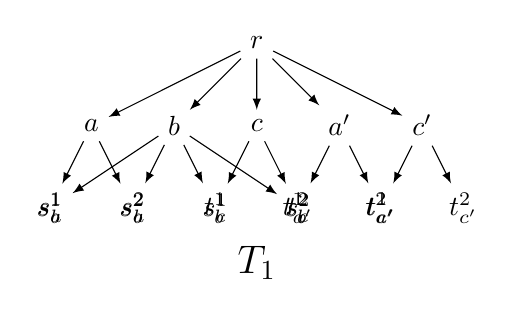
\begin{tikzpicture}[scale=0.7]
    \node (root) {$r$}
    child { node {$a$}
      child { node {$s_a^1$} }
      child { node {$s_a^2$} } }
    child { node {$b$}
      child { node {$s_b^1$} }
      child { node {$s_b^2$} }
      child { node {$t_b^1$} }
      child { node {$t_b^2$} } }
    child { node {$c$}
      child { node {$s_c^1$} }
      child { node {$s_c^2$} } }
    child { node {$a'$}
      child { node {$t_{a'}^1$} }
      child { node {$t_{a'}^2$} } }
    child { node {$c'$}
      child { node {$t_{c'}^1$} }
      child { node {$t_{c'}^2$} } } ;
    \node[draw=none] at (0,-4) {\Large $\Tone$} ;
  \end{tikzpicture}
  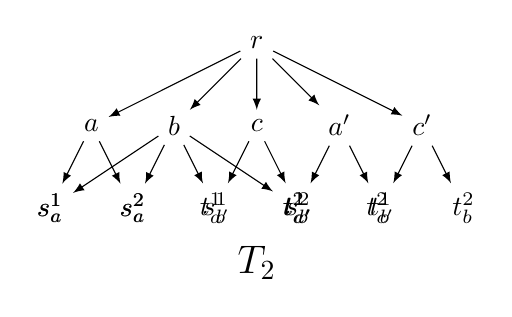
\begin{tikzpicture}[scale=0.7]
    \node (root) {$r$}
    child { node {$a$}
      child { node {$s_c^1$} }
      child { node {$s_c^2$} } }
    child { node {$b$}
      child { node {$s_a^1$} }
      child { node {$s_a^2$} }
      child { node {$t_{a'}^1$} }
      child { node {$t_{a'}^2$} } }
    child { node {$c$}
      child { node {$s_b^1$} }
      child { node {$s_b^2$} } }
    child { node {$a'$}
      child { node {$t_{c'}^1$} }
      child { node {$t_{c'}^2$} } }
    child { node {$c'$}
      child { node {$t_b^1$} }
      child { node {$t_b^2$} } } ;
    \node[draw=none] at (0,-4) {\Large $\Ttwo$} ;
  \end{tikzpicture}
\end{comment}
  \caption[Reduction from 3D matching]{The trees $\Tone$ (left) and $\Ttwo$ (right)
    given instance $H$ of 3-dimensional matching with $A=\{a,a'\}$,
    $B=\{b\}$ and $C=\{c,c'\}$ and $\cT=\{s = \{a,b,c\}, ~ t =
    \{a',b,c'\}\}$.}
  \label{fig:reductionNP}
\end{figure}

\begin{proof}
  Reduction from 3-bounded 1-common 3-dimensional matching.  We are
  given an instance $H$ of 3-dimensional matching consisting of a set
  $\cT$ of $m$ triples $(a,b,c)$ over the disjoint sets $A$, $B$, $C$.
  We construct two trees $\Tone$ and $\Ttwo$ each with $|A| + |B| +
  |C| + 6m + 2$ vertices, for which the rearrangement distance
  $d(\Tone, \Ttwo) \leq 3n + 6(m-n)$ if and only if $H$ has a
  3-dimensional matching of size $n$.

  Consider such an instance $H$ of 3-dimensional matching.  In the
  construction, the trees $\Tone$ and $\Ttwo$ each have a root vertex
  $r$, and a vertex for every element of $A$, $B$ and $C$ --- each of
  which have $r$ as the parent.  For each triple $t=(a,b,c)\in
  \mathcal{T}$, we add a pair $S_{t,v} = \{t_v^1, t_v^2\}$ of
  (uniquely labelled) children for each $v \in \{a,b,c\}$ of the
  triple $t$.  In $\Ttwo$, we add the pairs $S_{t,v}$ to each of these
  three vertices, but cyclically shifted, with respect to $\Tone$,
  i.e., we add $S_{t,a}$ to $b$, $S_{t,b}$ to $c$, $S_{t,c}$ back to
  $a$ again.
  
  By construction of the trees \Tone{} and \Ttwo, we can assume that
  each permutation involves only nodes of the universal set $U = A
  \cup B \cup C$ or only nodes representing triples of $\cT$ (never a
  mixture of the two).  Moreover, no node of the universal set $U$ is
  involved in a link-and-cut operation, since changing its parent
  would mean that the new parent is a node that is not $r$, which is
  not optimal.  Finally, any permutation of nodes representing the
  triples can be replaced by a sequence of link-and-cut operations
  with the same cost.  The overall effect is that we can restrict
  ourselves to sequences of operations consisting of permutations of
  nodes of $U$ followed by link-and-cut operations on nodes
  representing the triples.

  Let $M$ be a 3-dimensional matching of $H$.  Then for each triple
  $t=(a,b,c) \in M$ apply the permutation $(a,b,c)$ to $\Tone$.  After
  this permutation, each node node $S_{t,v}$ (with $v\in \{a,b,c\}$)
  has $v$ as its new parent.  Since $M$ is a matching, those
  permutations are independent.  For each triple $t=(a,b,c) \notin M$,
  apply a link-and-cut operation to each node in $S_{t,v}$ (with $v\in
  \{a,b,c\}$) so that its new parent is $v$.  It is immediate to
  notice that the resulting tree is exactly $T_2$ and that the overall
  cost of the operations is $3n + 6(m - n)$.\gdv{Requires inverting
    \Tone and \Ttwo}\murray{I think the slight change made in this
    paragraph avoids this requirement (or am I missing something?)}
  
  Let us now consider a sequence $S$ of permutations followed by
  link-and-cut operations that transforms $\Tone$ to $\Ttwo$.  We will
  show how to obtain a sequence of permutations followed by
  link-and-cut operations that is not more expensive than $S$, and
  where the permutations have cost 3, are disjoint, and each
  permutation involves exactly the elements of a triple of $\cT$.  By
  the first part of the proof, this suffices to prove the NP-hardness.

  First of all, no node is moved in two separate link-and-cut
  operations.  Moreover, either all nodes in a pair
  $S_{t,v}$,\murray{is this right, GDV?} for some $t, v$, are moved
  with link-and-cut operations, or none of them is moved.

  Let $X$ be the set of pairs $S_{t,v}$ such that no node is moved
  with link-and-cut operations.  By the construction of our reduction
  and the fact that the instance is 3-bounded and 1-common, the triple
  $t$ associated with each pair $S_{t,v}$ of $X$ appears in exactly
  one permutation.\murray{not sure if I follow this statement} Let $P$
  be the set of such triples.  Hence replacing the permutation with a
  sequence of permutations, one for each triple in $P$, results in a
  sequence where the permutations have cost 3, are disjoint, and each
  permutation involves exactly the elements of a triple of $\cT$.

  We have to modify the link-and-cut operations involving the sets
  that are not in $X$, but no new operation is added, completing the
  proof.\gdv{I don't like the proof, but it shows clearly that cycles
    of the movement graphs corresponds to triples in the
    instance. Hence we can remove the movement graph.}\murray{removed
    the movements graph.}

%
  % operations of total size $d(\Tone,\Ttwo)$ will consist of a
  % permutation followed by a sequence of link-and-cut operations.
  % Observe that any permutation involves for each cycle $\cC_t$ an
  % edge, two edges or all three edges.  Now, the rearrangement distance
  % aims to solve cycles in the movements graph in the sense that after
  % the operations, the movements graph has no edges.  Observe that
  % given a cycle $\cC_t$ of the movements graph $G$, then the minimum
  % cost rearrangement to solve $\cC_t$ consists of applying a
  % permutation of size $3$ involving the three vertices of the cycle,
  % thus of total cost $3$.  Observe that two cycles sharing a common
  % vertex cannot both be solved by a permutation that is a cyclic shift
  % of the vertices of the cycle, that is they cannot be both solved
  % with cost $3$.  Moreover, permutations of vertices cannot solve more
  % than one vertex of a cycle $\cC_t$ if it is not a cyclic shift of
  % the vertices of $\cC_t$, as cycles do not share edges.  In case of a
  % cyclic shift of two vertices of $\cC_t$, (1) a permutation of size
  % $2$ and then four link-and-cut operations are required. If instead
  % (2) at most a single vertex of $\cC_t$ is involved in a permutation,
  % then six link-and-cut operations are required.  We now detail how
  % this implies that $d(\Tone, \Ttwo) \leq 3n + 6(m- n)$ if and only if
  % $H$ has a 3-dimensional matching of size $n$.
%
  % ($\Rightarrow$) Assume that $d(\Tone, \Ttwo) \leq 3n + 6(m - n)$.
  % By the above observation on how cycles of the movements graph $G$
  % are solved by the sequence of permutations, cases (1) and (2) for
  % solving cycles have the same cost equal to $6$.  Thus the only
  % possible way to have a rearrangement distance less than or equal to
  % $3n + 6 (m- n) $ is by taking $n$ disjoint cycles solved by the
  % permutation operation of cost $3$. This implies a 3-dimensional
  % matching of size $n$.
\end{proof}

\subsection{A 4-Approximation Algorithm for Binary Trees}\label{sec:approxbinary}

We start by giving a lemma which states that when we
apply a permutation to the labels of $T_1$ obtaining $T'_1$, the size
of the resulting family partition $\cP'$ cannot increase or decrease
too much with respect to the size of $\cP$.

\begin{lemma}
  \label{lemma:partition}
  Given trees $T_1$ and $T_2$ with corresponding active set $\cX$ and
  family partition $\cP$, if $T_1'$ is the tree (isomorphic to $T_1$)
  resulting from the application of permutation $\pi$ of the labels of
  $T_1$, and $\cX'$ and $\cP'$ are the active set and the family
  partition of $T_1'$ and $T_2$, respectively, then $|\cP| - 2|\pi|
  \le |\cP'| \le |\cP| + 2|\pi|$.
\end{lemma}

\begin{proof}
  Let $a$ be some label of $T_1$ which has been perturbed by
  permutation $\pi$, i.e., $\pi(a) = b \ne a$.  The new family
  partition $\cP'$ is obtained from $\cP$ by means of deletions,
  insertions and substitutions of subsets.  The crucial observation is
  that such an operation will only affect the \emph{neighborhood} of
  $a$, namely the (possibly empty) set of its children $c_{T_1}(a)$
  and its parent $p_{T_1}(a)$ in $T_1$. 
  Let us split the children into three sets:
  \begin{itemize}
  \item $c_{T_1}(a) \cap \cP_{(a,b)}$, that is the children that are in $\cP_{(a,b)}$. 
  Notice that $\pi$ makes $b$ the new parent of all nodes in $c_{T_1}(a) \cap \cP_{(a,b)}$, therefore $\cP_{(a,b)}$ will be removed;
  \item $c_{T_1}(a) \cap \cP_{(a,a)}$, that is the children that are not in the family partition. The new set $\cP'_{(b,a)}$ will be created with those children;
  \item $c_{T_1}(a) \setminus \cP_{(a,b)}\setminus \cP_{(a,a)}$, that is the children that are not in $\cP_{(a,b)}$. 
  A generic children $v\in c_{T_1}(a) \setminus \cP_{(a,b)}$ belongs to a set  $\cP_{(a,c)}$, thus $\cP_{(a,c)}$
    will be replaced by $\cP'_{(b,c)}$ in $\cP'$.
  \end{itemize}

  Overall, for each label $a$, at most one set of the family partition will be created and at most one will be deleted.
  Consider now the possible effects of $\pi$ on $p_{T_1}(a)$. Notice that $a\in \cP_{(p_{T_1}(a),p_{T_2}(a))}$ and $a\in \cP'_{(p_{T_1}(b),p_{T_2}(a))}$.
  Therefore $\cP_{(p_{T_1}(a),p_{T_2}(a))}$ is the only set of the family partition that might be deleted, while $\cP'_{(p_{T_1}(b),p_{T_2}(a))}$ is the only set that might be created.


  In summary, $\cP'$ is obtained from $\cP$ with up to two deletions
  and two additions of sets in the family partition (and an unbounded number of replacements) for each label
  involved in the permutation $\pi$, thus the result follows.
\end{proof}

In the special case where one of the trees, e.g., $T_1$, is
\emph{binary}, that is, each node has up to two children, we have the
following lemma connecting link-and-cut and rearrangement distance.

\begin{lemma}
  \label{lemma:apxbin}
  Given $T_1$ a binary tree, $T_2$ any tree, we have that
  $d_{\ell}(T_1,T_2)\le 4\cdot d(T_1,T_2)$.
\end{lemma}

\begin{proof}
  Suppose that $T_2$ is optimally obtained from $T_1$ by applying a
  permutation $\pi$ of the labels followed by a number of link-and-cut
  operations.  Let $T'_1$ be the tree
  resulting from the application of permutation $\pi$ of the labels of
  $T_1$, $\cX'$ and $\cP'$ the active set and family partition of
  $T'_1$ and $T_2$, respectively.  By the construction of the family
  partition, the optimal number of link-and-cut operations to obtain
  $T_2$ from $T'_1$ is at least $|\cP'|$; we thus have that
  $d(T_1,T_2)= |\pi| + |\cX'| \ge |\pi| + |\cP'| $. Moreover, Lemma
  \ref{lemma:partition} says that $|\pi|\ge \frac{|\cP|-|\cP'|}{2}$,
  thus $d(T_1,T_2)\ge \frac{|\cP|-|\cP'|}{2} + |\cP'| =
  \frac{|\cP|}{2} + \frac{|\cP'|}{2} \ge \frac{|\cP|}{2}$.  Now, since
  $T_1$ is binary, each set in the family partition $\cP$ consists of
  up to two elements (the elements of $\cP_{(x,y)}$ are the ones among
  the children of $x$ in $T_1$ that becomes the children of $y$ in
  $T_2$, thus they cannot be more than the number of children of
  $x$). It follows that $|\cX|=d_{\ell}(T_1,T_2)\le 2\cdot|\cP|$,
  hence $d(T_1,T_2)\ge \frac{d_{\ell}(T_1,T_2)}{4}$.
\end{proof}

Importantly, we note that Lemma \ref{lemma:apxbin} states that the
link-and-cut distance algorithm provides a 4-approximation for
the rearrangement distance when at least one of the trees involved is
binary.
We now show that we can compute the link-and-cut distance between
two trees in linear time by showing that the family partition can be
built in linear time.

\begin{lemma}
  \label{lemma:edge}
  The link-and-cut distance $d_{\ell}(T_1,T_2)$ between trees $T_1$
  and $T_2$ each labelled by $[n]$ can be computed in time $O(n)$.
\end{lemma}

\begin{proof}
  Since the link-and-cut distance is $|\cX|$, it suffices to
  demonstrate that the family partition $\cP$ can be built in time
  $O(n)$.  The procedure is as follows: we first do a DFT of tree
  $T_1$, building an array $p_{T_1}(v)$ of the parents in $T_1$,
  indexed by the child $v$.  We build the same array $p_{T_2}(v)$ for
  tree $T_2$.  Then we go through the set $[n]$ of labels, in some
  order: at each label $v$, should $p_{T_1}(v) = u \ne p_{T_2}(v) =
  w$, we add $v$ to $\cP_{(u,w)}$ of the family partition $\cP$.  Then
  we just sum up the sizes of the non-empty subsets $\cP_{(u,w)}$ of
  $\cP$ in order to obtain $|\cX| = d_{\ell}(T_1,T_2)$.  Clearly each
  tree traversal can be done in time $O(n)$, as both $\Tone$ and $\Ttwo$ have $n$ vertices.  In going through the labels, for each label
  $v$, we either add or do not add the single vertex $v$ to $\cP$, and
  so this procedure takes time $O(n)$.
\end{proof}

We thus have the following corollary from Lemma~\ref{lemma:apxbin}
and Lemma~\ref{lemma:edge}.

\begin{corollary}
  \label{corollary:apx}
  There exists a linear time $4$-approximation algorithm for the
  rearrangement distance problem for binary trees.
\end{corollary}

\subsection{A General Constant-Factor Approximation Algorithm}\label{sec:approxtree}

In what follows we do not make any assumptions on the degrees of $\Tone$ and $\Ttwo$.
We will actually consider the rearrangement distance generalized to forests, $\tilde d(\Fone,\Ftwo)$ (see the definition at Section~\ref{sec:preliminariestree}), and show how to approximate it within
a constant factor. This allows us to approximate $d(\Tone,\Ttwo)$ within a constant factor
using the following procedure.
First, we add $n$ leaves $n+1,n+2,\ldots,2n$ attached to the (identical) roots of $\Tone$ and $\Ttwo$ to obtain $\Tone'$ and $\Ttwo'$, respectively.
We call the resulting trees \emph{anchored}. Because $\Tone$ and $\Ttwo$ are assumed to have the
same root that cannot be permuted, we have $d(\Tone,\Ttwo)=d(\Tone',\Ttwo')$.
We claim that $\tilde d(\Tone',\Ttwo')=d(\Tone',\Ttwo')$.

\begin{lemma}
\label{lem:atmost}
For any two anchored trees $\Tone$ and $\Ttwo$, $\tilde{d}(\Tone,\Ttwo)= d(\Tone,\Ttwo)$.
\end{lemma}
\begin{proof}
Consider a sequence $s$ of link-and-cut and permutation operations
that transforms $\Tone$ into $\Ttwo$. We convert it into a sequence $s'$ of cut and permutation operations by simply
replacing every link-and-cut operation $v\,|\,u\rightarrow w$ with a cut operation $(v\dagger u)$. Let $\Tone'$ be the forest
obtained after applying $s'$ on $\Tone$. We claim that $\Tone' \sim \Ttwo$. Consider any $v\in [n]$.
Because we can assume that the permutation operation precedes all the link-and-cut operations in $s$,
if $p_{\Tone'}(v) \neq \bot$ then we must have $p_{\Ttwo}(v)=\bot$ or $p_{\Tone'}(v)=p_{\Ttwo}(v)$, as
$p_{\Tone'}(v)$ is the same as the parent of $v$ after applying $s$ on $\Tone$. This
shows that indeed $\Tone' \sim \Ttwo$, and so $\tilde{d}(\Tone,\Ttwo) \leq d(\Tone,\Ttwo)$.

For the other direction, we use the assumption that $\Tone$ and $\Ttwo$ are anchored trees on $2n$ nodes:
in both trees $r$ is the root and there are $n$ leaves $n+1,n+2,\ldots,2n$ attached to $r$.
Observe that $\tilde d(\Tone,\Ttwo)<n$. We claim that an optimal sequence of cut and permutation operations
doesn't permute $r$. Assume otherwise, then for every $u=n+1,n+2,\ldots,n$ either $u$
is also permuted, or we have a cut operation $(u \dagger r)$, so the size of the sequence must be at least $n$.
Now, let $s$ be an optimal sequence consisting of a permutation $\pi$ and then some cut operations,
and let $\Tone''$ be the tree obtained after applying $s$ on $\Tone$.
We obtain a sequence $s'$ of link-and-cut and permutation operations from $s$ as follows.
For every $v\in [n]$, if $p_{\Tone''}(v) = \bot$ and $p_{\Ttwo}(v)\neq \bot$, we locate the cut operation $(v\dagger u)$ in $s$ (there must be such operation, as $\Tone$ and $\Ttwo$ have the same root that is not permuted). In $s'$, we replace this operation with $v\,|\,u\rightarrow w$, where $w=p_{\Ttwo}(v)$.
Additionally, we reorder all link-and-cut operations to ensure that $w$ is not a descendant of $v$, which can be guaranteed by considering $v$ in the decreasing order of their levels in $\Ttwo$.
Let $\Tone'$ be the result of applying $s'$ on $\Tone$, and consider any $v\in [n]$.
If $p_{\Tone''}(v) \neq \bot$ and $p_{\Ttwo}(v) \neq \bot$ then $p_{\Tone'}(v)=p_{\Ttwo}(v)$
because $\Tone'' \sim \Ftwo$, and if $p_{\Tone''}(v) = \bot$ and $p_{\Ttwo}(v)\neq \bot$ then
$p_{\Tone'}(v)=p_{\Ttwo}(v)$ by the choice of $w$.
This shows that $s'$ transforms $\Tone$ into $\Ttwo$, thus $d(\Tone,\Ttwo) \leq \tilde{d}(\Tone,\Ttwo)$.
\end{proof}

\begin{figure}[t]
    \centering
   \includegraphics[width=.9\linewidth]{Fig/approx.pdf}
   \caption{The four steps of the approximation algorithm.}
    \label{fig:approx}
\end{figure}

We can thus approximate $\tilde{d}(\Tone',\Ttwo')$ within a constant factor to obtain a constant factor
approximation of $d(\Tone,\Ttwo)$. In the remaining part of this section we design an approximation algorithm
for $\tilde{d}(\Fone,\Ftwo)$, where $\Fone$ and $\Ftwo$ are two arbitrary forests.

We start with describing the notation. Consider two forests $\Fone$ and $\Ftwo$.
For every $i\in [n]$, let $a[i]\in[n]$ be the parent of a non-root node $i$ in $\Fone$, and $a[i]=0$ if $i$ is a root in $\Fone$. Formally,
$a[i]=p_{\Fone}(i)$ when $p_{\Fone}(i)\neq \bot$ and $a[i]=0$ otherwise;
$b[i]$ is defined similarly but for $\Ftwo$.
We think of $a$ and $b$ as vectors of length $n$.

The algorithm consists of four steps, with step $j$ transforming forest $\Fone^{j-1}$ into $\Fone^{j}$ by performing
$\alg(j)$ operations, starting from $\Fone^{0}=\Fone$.
We will guarantee that $\alg(j) = \cO(\tilde{d}(\Fone^{j-1},\Ftwo))$.
Then, by triangle inequality and symmetry,
$\tilde{d}(\Fone^{j},\Ftwo)\leq \tilde{d}(\Fone^{j-1},\Fone^{j})+\tilde{d}(\Fone^{j-1},\Ftwo)\leq
\alg(j)+\tilde{d}(\Fone^{j-1},\Ftwo)=\cO(\tilde{d}(\Fone^{j-1},\Ftwo))$, so by induction $\tilde{d}(\Fone^{j},\Ftwo)=\cO(\tilde{d}(\Fone,\Ftwo))$.
Consequently, $\alg(j) = \cO(\tilde{d}(\Fone,\Ftwo))$, making the overall cost $\sum_{j}\alg(j) = \cO(\tilde{d}(\Fone,\Ftwo))$.
In the $j$-th step of the algorithm $a[i]$ refers to the parent of $i$ in $\Fone^{j-1}$.
To analyse each step of the algorithm we will use the following two structures, the first of which is a streamlined version
of family partitions defined in~\ref{sec:preliminariestree}.


\begin{definition}[family partition of two forests]
\label{def:family}
Given two forests $\Fone$ and $\Ftwo$, their \emph{family partition}
$P(\Fone,\Ftwo)$ is the set $\{ (a[i],b[i]) : a[i],b[i]\neq 0~\land~a[i] \neq b[i] \}$.
\end{definition}

\begin{definition}[migrations graph]
\label{def:migrations}
Given two forests $\Fone$ and $\Ftwo$, the \emph{migrations graph}
$MG(\Fone,\Ftwo)$ consists of edges $ \{ (i,j) : a[i],a[j],b[i],b[j]\neq 0~\land~a[i]=a[j]~\land~b[i]\neq b[j] \} $.
\end{definition}

For a multiset $S$, let $|S|$ denote its cardinality, that is, the sum of multiplicities of all distinct elements of $S$.
The mode of $S$, denoted $\mode(S)$, is any element $s\in S$ with the largest multiplicity $\freq_{S}(s)$. We will use the following combinatorial lemma.

\begin{restatable}{lemma}{lempairs}
\label{lem:pairs}
Given any multiset $S$, let $f=\min\{|S|-\freq_{S}(\mode(S)),\lfloor |S|/2\rfloor\}$. All $|S|$ elements of $S$
can be partitioned into $f$ pairs $(x_{1},y_{1}),\ldots,(x_{f},y_{f})$,
$x_{i}\neq y_{i}$, for every $i\in [f]$, and the remaining $|S|-2f$ elements.
\end{restatable}

\begin{figure}[ht]\hspace{-1.2cm}
    \begin{subfigure}[c]{0.6\textwidth}
       \includegraphics[width=1\textwidth]{Fig/Lemma11.pdf}
       %\vspace{-8mm}
    \end{subfigure}
    \hspace{-3mm}
    \begin{subfigure}[c]{0.6\textwidth}
    %\vspace{1pt}
       \includegraphics[width=1\textwidth]{Fig/Lemma11_2.pdf}
       %\vspace{-8mm}
    \end{subfigure}
    \caption[Pairing of elements of a multiset]{Pairing in the case $f=|S|-\freq_{S}(\mode(S))$ (left) and $f=\lfloor |S|/2\rfloor$ (right).}
    \label{fig:pairing}
\end{figure}

\begin{proof}
Number the elements of $S$ so that $s_1=\ldots =s_{\freq_S(\mode(S))}=\mode(S)$ and all of the others are sorted and numbered from $\freq_S(\mode(S))+1$ to $|S|$ accordingly.
Then, if $f=|S|-\freq_{S}(\mode(S))$, pairs $(s_i,s_{|S|-i+1})$, $i\in [f]$ are s.t. $s_i\neq s_{|S|-i+1}$ (Figure~\ref{fig:pairing}, left); if $f=\lfloor |S|/2\rfloor$, pairs $(s_i,s_{\lfloor |S|/2\rfloor+i})$, $i\in [\lfloor |S|/2\rfloor]$ are s.t. $s_i\neq s_{\lfloor |S|/2\rfloor+i}$ (Figure~\ref{fig:pairing}, right).
\end{proof}

\subsection{Step 1}
Roughly speaking, the aim of the first step is to ensure that all nodes that might be possibly involved in a permutation, i.e.,
the nodes with different children in $\Fone$ and $\Ftwo$, are roots. This is so that we do not need to worry about the relationship
with their parents.
For every $i\in [n]$ such that $a[i]$ and  $b[i]$ are both defined and different, we cut
the edges from $a[i]$ and $b[i]$ to their parents in $\Fone$, thus making both of them roots.
In other words, for every $i$ such that $a[i],b[i]\neq 0$ and $a[i]\neq b[i]$, we cut edges $(a[i],a[a[i]])$ and $(b[i],a[b[i]])$.
The resulting forest $\Fone^1$ has the following property: for each $i\in [n]$ such that
the parents of $i$ in $\Fone^{1}$ and in $\Ftwo$ are both defined and different,
$a[a[i]]=a[b[i]]=\bot$.

The number of cuts in this step is by definition at most twice the size of the family partition $P(\Fone,\Ftwo)$.
By Lemma~\ref{lemma:partition} it follows immediately that $|P(\Tone,\Ttwo)| \leq 2d(\Tone,\Ttwo)$ for two trees $\Tone$ and $\Ttwo$.
We show that this still holds for forests and $\tilde{d}$: for completeness, we provide a self-contained proof.
%
\begin{restatable}{lemma}{lempartition}
\label{lem:activeset}
$|P(\Fone,\Ftwo)|  \leq 2\tilde{d}(\Fone,\Ftwo) $, implying $\alg(1)\le 4\tilde{d}(\Fone,\Ftwo)$.
\end{restatable}

\begin{proof}
It is enough to verify that applying a single cut operation might decrease the size of the family partition by at
most one, while applying a permutation operation $\pi$
might decrease the size of the family partition by at most $2s$, where $s=|\{ u : u \neq \pi(u) \}|$.

Consider a cut operation $(v \dagger u)$. The only change to $a$ is that $a[v]$ becomes $0$,
so indeed the size of the family partition might decrease by at most one.

Now consider a permutation $\pi$.
%Recall that the family partition is defined as
%\[ P=\{ (a[i], b[i]) : a[i] \neq 0~\land~b[i] \neq 0~\land~a[i] \neq b[i]\} . \]
After applying $\pi$, an edge $(i,a[i])$ becomes $(\pi(i),\pi(a[i]))$, making $\pi(a[\pi^{-1}(i)])$ the parent of $i$.
This transforms the family partition $P$ into
\[ P'=\{ (\pi(a[i]), b[\pi(i)]) : a[i] \neq 0~\land~b[\pi(i)] \neq 0~\land~\pi(a[i]) \neq b[\pi(i)]\} .\]
To lower bound the size of $|P'|$, we first focus on the subset of $P$ corresponding to the nodes that are fixed by $\pi$. We therefore define
\[ P_{f} = \{ (a[i], b[i]) : a[i] \neq 0~\land~b[i] \neq 0~\land~a[i] \neq b[i]~\land~\pi(i)=i\} . \]
By definition, we can equivalently rewrite $P_{f}$ as
\[ P_{f} = \{ (a[i], b[\pi(i)]) : a[i] \neq 0~\land~b[\pi(i)] \neq 0~\land~a[i] \neq b[\pi(i)]~\land~\pi(i)=i\} . \]
Now consider all pairs with the same second coordinate $y$ in $P_{f}$: $(x_{1},y),(x_{2},y),\ldots,(x_{k},y)$, where $x_{i}\neq y$ for every $i\in [k]$.
$P'$ contains all pairs $(\pi(x_{i}),y)$ such that $\pi(x_{i})\neq y$. If $\pi(y)=y$ then $\pi(x_{i})= y$ cannot
happen and $P'$ contains all pairs with the second coordinate $y$ from $P_{f}$;
otherwise, $P'$ contains all such pairs except possibly one. Overall, $|P'| \geq |P_{f}|-s$, and $|P_{f}| \geq |P|-s$ so indeed $|P'| \geq |P|-2s$.
\end{proof}

\begin{figure}[t]
    \centering
   \includegraphics[width=0.9\linewidth]{Fig/Fone_Ftwo.pdf}
    \caption[Family partition of two forests]{$\Fone$ and $\Ftwo$. The family partition is $P=\{(2,3), (2,7), (3,7), (7,3), (7,2)\}$.}
    \label{fig:trees}
\end{figure}

\begin{figure}\hspace{-1mm}
\centering
    \begin{subfigure}[b]{0.38\textwidth}
       \includegraphics[width=1\textwidth]{Fig/step1.pdf}
       \vspace{-3mm}
        \caption{$\Fone^1$}
        \label{fone1}
    \end{subfigure}
    ~~~~ %add desired spacing
    \begin{subfigure}[b]{0.38\textwidth}
       \includegraphics[width=1\textwidth]{Fig/step2.pdf}
       \vspace{-3mm}
        \caption{$\Fone^2$}
        \label{fone2}
    \end{subfigure}

    \begin{subfigure}[b]{0.38\textwidth}
       \includegraphics[width=1\textwidth]{Fig/step3.pdf}
      \vspace{-3mm}
        \caption{$\Fone^3$}
        \label{fone3}
    \end{subfigure}
    ~~~~
    \begin{subfigure}[b]{0.38\textwidth}
       \includegraphics[width=1\textwidth]{Fig/step4.pdf}
      \vspace{-3mm}
        \caption{$\Fone^4$}
        \label{fone4}
    \end{subfigure}

    \caption[The four steps of the approximation algorithm]{The forests obtained after Step 1 (\ref{fone1}), Step 2 (\ref{fone2}), Step 3 (\ref{fone3}) and Step 4 (\ref{fone4}).} \label{fig:forest}
\end{figure}

\begin{example}
\label{ex:step1}
Consider $\Fone$ and $\Ftwo$ depicted in Figure~\ref{fig:trees}. Step 1 consists of cut operations $(2\dagger1)$ (because, e.g., $a[4]\neq b[4]$ and $a[4]=2$), $(3\dagger1)$ (because $b[4]=3$) and $(7\dagger2)$ (because, e.g., $a[11]\neq b[11]$ and $a[11]=7$). The resulting forest $\Fone^1$ is shown in Figure~\ref{fone1}.
\end{example}

\subsection{Step 2}
Consider $u\in [n]$, and let $\children_{\Fone^{1}}(u)=\{v_{1},\ldots,v_{k}\}$.
We define the multiset $B(u)=\{b[v_{i}] : b[v_{i}]\neq 0 \}$ containing the parents in $\Ftwo$ of
the children of $u$ in $\Fone^{1}$.
Recall that $\mode(B(u))$ is the most frequent element of $B(u)$ (ties are broken arbitrarily).
We cut all edges $(v_{i},u)$ such that $b[v_{i}]\neq 0$ and $b[v_i]\neq \mode(B(u))$, and define, for each $u\in [n]$, its representative  $\rep(u)=\mode(B(u))$.
Intuitively, $\rep(u)$ is the node that might be convenient to replace $u$ with using a permutation.
Roughly speaking, in this step we get rid of all of the children of $u$ that would be misplaced after permuting $u$ and $\rep(u)$, for each $u\in[n]$. The resulting forest $\Fone^2$ has the following property: for each $u\in [n]$,
for any child $v$ of $u$ in $\Fone^{2}$, either $b[v]=0$ or $b[v]=\rep(u)$, i.e., the children of each node $u$ of $\Fone^2$ have all the same parent $\rep(u)$ in $\Ftwo$.

To bound the number of cuts in this step we first need a technical lemma relating the rearrangement distance of two
forests and the size of any matching in their migrations graph.

\begin{lemma}
\label{lem:opt}
Consider two forests $\Fone$ and $\Ftwo$ and their migrations graph $MG(\Fone,\Ftwo)$. For any matching $M$ in
$MG(\Fone,\Ftwo)$ it holds that $|M|\le \tilde{d}(\Fone,\Ftwo)$.
\end{lemma}

\begin{proof}
By definition, there is an edge between $i$ and $j$ in $MG(\Fone,\Ftwo)$ if and only if $a[i]=a[j]$, but $b[i]\neq b[j]$.
Let $M$ be any matching in $MG(\Fone,\Ftwo)$. If $|M| > 0$ then $\tilde{d}(\Fone,\Ftwo) \geq 1$,
so it is enough to show that, for a single operation transforming $\Fone$ into $\Fone'$,
the graph $MG(\Fone',\Ftwo)$ contains a matching $M'$ of size at least $|M|-s$, where $s=1$ for a cut operation and $s=|\{ u : u \neq \pi(u) \}|$ for a permutation operation $\pi$.

First, consider a cut operation $(v \dagger u)$. The only change in $MG(\Fone',\Ftwo)$ is removing
all edges incident to $v$. $M$ contains at most one edge incident to $v$, so we construct $M'$
of size at least $|M|-1$ from $M$ by possibly removing a single edge.
Second, consider a permutation operation $\pi$: we construct $M'$
from $M$ by removing every edge $(v,w)$ such that $v \neq \pi(v)$ or $w \neq \pi(w)$. Because
there is at most one edge incident to every $u$ such that $u \neq \pi(u)$, $M'$ contains
at least $|M|-s$ edges. $M'$ is a matching in $MG(\Fone',\Ftwo)$, as for every $(v,w)\in M'$
we have $p_{\Fone'}(v)=p_{\Fone}(v)$ and $p_{\Fone'}(w)=p_{\Fone}(w)$.
\end{proof}

\begin{lemma}
\label{lem:step2}
$\alg(2)\le 2\tilde{d}(\Fone^1,\Ftwo)$.
\end{lemma}

\begin{proof}
We consider each $u\in [n]$ separately. Let $m=\freq_{B_{u}}(\mode(B_u))$ and
$MG_{u}$ be the subgraph of $MG(\Fone^{1},\Ftwo)$ induced by $B_{u}$. We will first construct
a matching of appropriate size in every $MG_{u}$.
%
We cut every $(v_{i},u)$ such that $b[v_{i}]\neq 0$ and $b[v_{i}] \neq \mode(B_{u})$,
making $|B_{u}|-m$ cuts. Let $f=\min(|B_{u}|-m,\lfloor |B_{u}|/2\rfloor)$.
By Lemma~\ref{lem:pairs}, we can partition a subset of $B_{u}$
into $f$ pairs $(b[v_{i}],b[v_{j}])$ such that $b[v_i]\neq b[v_j]$. We add
every edge $(v_{i},v_{j})$ to the constructed matching. We claim that
$|B_{u}|-m \leq 2f$. This holds because $|B_{u}|-m \leq 2(|B_{u}|-m)$
and $|B_{u}|-m \leq |B_{u}|-1 \leq 2\lfloor |B_{u}/2|\rfloor$ for nonempty $B_{u}$.

We take the union of all such matchings to obtain a single matching $M$.
As argued above, the total number of cuts is at most $2|M|$.
Together with Lemma~\ref{lem:opt}, this implies that $\alg(2)\le 2|M| \le 2\tilde{d}(\Fone^1,\Ftwo)$.
\end{proof}

\begin{example}
\label{ex:step2}
Consider again $\Fone$ and $\Ftwo$ of Figure~\ref{fig:trees}.  $B(7)=\{3,3,3,2,7\}$, thus we cut $(14\dagger7)$ and $(15\dagger7)$. $B(2)=\{3,3,7\}$, implying  $(6\dagger2)$.
The resulting $\Fone^2$ is shown in Figure~\ref{fone2}.
\end{example}

\subsection{Step 3}
If after Step 2 all of the children of a node $u$ of $\Fone$ have the same parent $\rep(u)$ in $\Ftwo$, it still may be the case where $\rep(u)=\rep(v)$ with $u\neq v$, i.e., all of the children of two distinct nodes of $\Fone$ have the same parent in $\Ftwo$.
In this case, it is not clear how to choose whether to replace $u$ or $v$ with $\rep(u)=\rep(v)$ in a permutation.
This step aims at resolving this situation by cutting the ambiguous edges.

Consider thus $u\in [n]$, and let $\children_{\Ftwo}(u)=\{v_{1},v_{2},\ldots,v_{k}\}$.
We define the multiset
$B'(u)=\{ a[v_{i}] : a[v_{i}] \neq 0 \}$ containing the parents in $\Fone^{2}$ of the children of $u$ in $\Ftwo$. We
cut all edges $(v_{i},a[v_{i}])$ such that $a[v_{i}]\neq 0$ and $a[v_{i}]\neq \mode(B'(u))$, breaking ties arbitrarily, and define $\rep'(u)=\mode(B'(u))$.
The resulting forest $\Fone^{3}$ has
the following property: for each $u\in [n]$,
for any child $v$ of $u$ in $\Ftwo$, we have $a[v])=\bot$ or $a[v]=\rep'(u)$.

We observe that the number of cuts performed by the above procedure is the same as if we had applied
Step 2 on $\Ftwo$ and $\Fone^{2}$. Therefore, Lemma~\ref{lem:step2} implies the following.

\begin{lemma}
\label{lem:step3}
$\alg(3)\le 2\tilde{d}(\Fone^2,\Ftwo)$.
\end{lemma}

\begin{example}
\label{ex:step3}
Consider again $\Fone$ and $\Ftwo$ of Figure~\ref{fig:trees}.
We have $B'(3)=\{2,2,7,7,7\}$, we thus cut $(4\dagger2)$ and $(5\dagger2)$.
The resulting forest $\Fone^3$ is shown in Figure~\ref{fone3}.
\end{example}

\paragraph{Step 4}

We summarize the properties of $\Fone^{3}$ and $\Ftwo$:
\begin{enumerate}
\item For each $u\in [n]$ such that $a[u],b[u]\neq 0$ and $a[u]\neq b[u]$, $a[u]$ and $b[u]$ are roots in $\Fone^{3}$.\label{prop:one}
\item For each $u\in [n]$ we can define $\rep(u)\in [n]$ in such a way that, for any child $v$ of $u$ in $\Fone^{3}$, we have $b[v]=0$ or $b[v]=\rep(u)$.\label{prop:two}
\item For each $u\in [n]$ we can define $\rep'(u)\in [n]$ in such a way that, for any child $v$ of $u$ in $\Ftwo$, we have $a[v]=0$ or $a[v]=\rep'(u)$.\label{prop:three}
\end{enumerate}
To finish the description of the algorithm, we show how to find a permutation operation $\pi$ of size $\cO(\tilde{d}(\Fone^{3},\Ftwo))$
that transforms $\Fone^{3}$ into $\Fone^{4}$ such that $\Fone^{4} \sim \Ftwo$.

For every $u$ such that $a[u],b[u]\neq 0$ and $a[u]\neq b[u]$, we require that $\pi(a[u])=b[u]$.
Due to Property~\ref{prop:one}, for every such $u$ we have ensured that $a[u]$ and $b[u]$ are roots
of $\Fone^{3}$. So, if we can find a permutation $\pi$ that satisfies all the requirements and does not perturb the non-roots
of $\Fone^{3}$, then it will transform $\Fone^{3}$ into $\Fone^{4}$ such that $\Fone^{4}\sim \Ftwo$.
Furthermore, if for every $x$ perturbed by $\pi$ there exists $u$ such that
$a[u],b[u]\neq 0$ and $a[u]\neq b[u]$ with $x=a[u]$ or $x=b[u]$ then by Lemma~\ref{lem:activeset}
$|\pi| \leq 2|P(\Fone^{3},\Ftwo)| \leq 4\tilde{d}(\Fone^{3},\Ftwo)$ as required.

To see that there indeed exists such $\pi$, observe that due to Property~\ref{prop:two}
there cannot be two requirements $\pi(x)=y$ and $\pi(x)=y'$ with $y\neq y'$.
Similarly, due to Property~\ref{prop:three} there cannot be two requirements $\pi(x)=y$ and $\pi(x')=y$ with $x\neq x'$.
Thinking of the requirements as a graph, the in- and out-degree of every node is hence at most 1, so we can add extra edges to obtain a collection of cycles defining a permutation $\pi$ that does not perturb the nodes not participating in any requirement.

\begin{example}
Consider $\Fone$ and $\Ftwo$ of Figure~\ref{fig:trees}. $\pi=(3~7)$ transforms $\Fone^3$ into $\Fone^4\sim\Ftwo$.
The final $\Fone^{4}$ is shown in  Figure~\ref{fone4}.
\end{example}

\section{Fixed-parameter algorithms}
\label{sec:fixedpar}

This section is devoted to showing that computing the rearrangement
distance between trees $T_{1}$ and $T_{2}$ is fixed-parameter
tractable, essentially via the bounded search tree
technique~\cite{ParameterizedComplexity}.  In this case, we denote with $k$ the optimum rearrangement deistance: in time $O((4k)^{2k^{2}}n)$ we (1)
determine if $d(T_{1}, T_2)\le k $ and, if this is the case, (2) find
the minimum sequence of operations transforming $T_{1}$ into $T_{2}$.

Recall that we can consider only sequences of operations transforming $T_{1}$ into $T_{2}$ so that all
permutations precede the link-and-cut operations.  Let $T^{*}$ be a
tree obtained from $T_{1}$ using only permutations and such that we
can optimally obtain $T_{2}$ from $T^{*}$ using only link-and-cut
operations.  Then $d(T_1,T_2) = d_{\pi}(T_{1}, T^{*}) +
d_{\ell}(T^{*}, T_{2})$.  
Since we can compute $d_{\ell}(T^{*}, T_{2})$ in linear
time (Lemma~\ref{lemma:algorithm-link-and-cut}).

Lemma~\ref{lemma:partition} shows that each permutation has only a limited effect on the number of sets of the family partition. 
Our algorithm consists of showing that
$d_{\pi}(T_{1}, T^{*})$ is related to the size of the family
partition.
Finding
such a tree $T^{*}$ is easier when we want to determine if the
rearrangement distance $d(T_1,T_2)$ is at most $k$.

\begin{algorithm}[bt!]
    \KwData{Two labeled trees $T_1$ and $T_2$}
    \KwResult{The sequence of operations transforming $T_1$ into $T_2$}
    $\cP \gets$ the family partition associated with the pair $(T_1, T_2)$\;
    \For{$k\gets 1$ to $2|\cP|$}{%
        \ForEach{tree $T^*$ that can be obtained from $T_1$ with a sequence $S_{Pi}$ of at most $k$ permutations}{%
            $k_1\gets d_{\Pi}(T_1, T^*)$\;
            % \If{$T^* = T_2$}{%
            %     \Return $S_{\Pi}$
            % }
            $\cP_1 \gets$ the family partition associated with the pair $(T^*, T_2)$\;
            $S_{\ell}\gets $ the optimal sequence of link-and-cut operations transforming $T^*$ into $T_2$\;
            % \ForEach{tree $T$ that can be obtained from $T^*$ with a sequence $S_{\ell}$ of at most $k - k_1$ link-and-cut operations}{%
            \If{$k_1 + | S_{\ell} | \le k$}{%
                    \Return the concatenation $S_{\Pi} S_{\ell}$
                }
            % }
        }
    }

    \caption{Fixed parameter algorithm for the rearrangement distance}
    \label{alg:fixed-parameter}
\end{algorithm}


In fact, a consequence of Lemma~\ref{lemma:partition} is that
$d(T_{1}, T_2) \geq d_{\pi}(T_{1}, T^{*})\geq |\cP|/2 $, where $\cP$
is the family partition associated with $T_{1}$ and $T_{2}$.  Notice
that any sequence of operations that transforms $T_{1}$ into $T_2$
also transforms $\cX$ into the empty set, and thus $\cP$ into the empty
partition. The next lemma states that each operation in an optimal sequence strictly decreases the size of the family partition; this allows us to bound the size of the search tree in terms of the size of the family partition.

\begin{lemma}
  \label{lemma:always-smaller-family-partition}
  Let $T_1$, $T_2$ be two trees and let $S$ be an optimal sequence of operations transforming $T_1$ into $T_2$.
  Let $\cP$, $\cP'$ be the family partitions before and after an operation of $S$.
  Then $|\cP| > |\cP'|$.
\end{lemma}

\begin{proof}
  The proof of Lemma~\ref{lemma:algorithm-link-and-cut} shows that each link-and-cut operation strictly decreases the size of the family partition, therefore we only need to consider permutations.


  Assume to the contrary that there exists an optimal sequence of operations that contains a permutation $\pi$ that does not decrease the size of the family partition.
  W.l.o.g. we can assume that $\pi$ is the first such permutation in the sequence of operation.
\end{proof}

Since $d(T_{1}, T_2) \geq |\cP|/2 $, the first step of our algorithm
is to compute the family partition $\cP$ of $T_{1}$ and $T_{2}$ and
verify that $k\ge |\cP|/2$.  If that inequality is not satisfied,
then, since as stated above $d_\pi(T_{1}, T^{*}) \geq |\cP|/2 $, it
would follow that $d(T_{1}, T_2) > k $.  Hence we can focus on the
instances where $k\ge |\cP|/2$, that is $|\cP|\le 2k$.  Since the
family partition is sufficiently small, we can compute all sequences
of permutations of at most $k$ labels of $\cX$ in time
$O((4k)^{2k^{2}})$.  In fact, each of the permutations involves one of
the $2^{2k}$ subsets of vertices of $\cX$, and there can be at most
$(2k)!$ permutations of a set of $2k$ elements.  Overall there are at
most $\left(2^{2k}(2k)!\right)^{k}$ such sequences: it is trivial to
organize them in a search tree that can be generated and traversed in
linear time, and some crude upper bound results in the desired time
bound.  Let $\mathcal T$ be the set of trees that are obtained by
applying to $T_{1}$ the sequence of operations corresponding to a node
of the search tree.

The second part of our algorithm is to compute $d_{\ell}(T, T_{2})$ for
each tree in $T \in \cT$, which, by Lemma~\ref{lemma:edge}, requires
$O(n)$ time for each tree, keeping track of the tree $T^{*}$
minimizing $d_{\pi}(T_{1}, T^{*}) + d_{\ell}(T^{*}, T_{2})$.  The algorithm
has therefore $O((4k)^{2k^{2}}n)$ time complexity.

\bibliographystyle{plain}
\bibliography{references}

\end{document}
